The modelling systematic uncertainties include the 
uncertainties due to theoretical cross-section calculations
and accpetance. The former only affects the normalisation of the
samples, and is applied on all MC backgrounds; the later
affects both the expected event yields and the shape of
kinematic distributions, and therefore the MVA discriminant output
shapes. In order to disentangle these effects, the 
impact from shape variation is considered 
separately from the normalisation effect,
as it does not change the amount of expected events.
The shape uncertainties are derived comparing the 
distributions of several kinematic variables or MVA 
discriminant output of the alternative samples to the ones of the nominal sample. 
The comparison is done by taking the normalised distributions 
(to exclude the normalisation effects that are 
considered separately) and calculating the ratio of 
the alternative and nominal number of events bin per bin. 

Acceptance uncertainties for $t\bar{t}$, $Z$+heavy flavour jets, 
single-top ($Wt$-channel), ttH and ZH are estimated in the SR and CR, 
using the nominal and alternative MC simulated samples. 
The acceptance uncertainties on minor 
backgrounds ($Z$+light flavour jets, $W$+jets, and di-boson) 
are taken from Ref.\cite{ATLAS-CONF-2020-006}, as 
described in Section~\ref{subsec:uncertainties_minor_bkgs}. 

The normalisation acceptance uncertainties are derived comparing the 
acceptance obtained for each alternative sample 
to the nominal acceptance:

\begin{equation}
    \sigma_{A}= \frac{A_\text{var} - A_\text{nom}}{A_\text{nom}} = \frac{N_\text{var}-N_\text{nom}}{N_\text{nom}},
    \label{eq:acceptance_unc}
\end{equation}
where $A_\text{var}$ ($A_\text{nom}$) is the acceptance of the 
variation (nominal) sample and  $N_\text{var}$ ($N_\text{nom}$) 
is the expected events yields of the variation (nominal) sample. 
Acceptance uncertainties on the normalisation of the 
backgrounds are applied in all regions and 
treated as correlated across regions except for the 
$t\bar{t}$ and \ZHF\ backgrounds whose normalisations 
are left unconstrained (floated) in the global likelihood fit. 
For these two processes, a relative acceptance uncertainty is needed
to take into account the correlation.
The relative acceptance uncertainty is estimated
from the comparison of the relative amount of events predicted by the 
alternative model in one region `$i$' with 
respect to another region `$j$' and the same fraction 
in the nominal model:
\begin{equation}
\sigma_{A^i/A^j}= \frac{\frac{A_{var}^i}{A_{var}^j} - \frac{A_{nom}^i}{A_{nom}^j}}
{\frac{A_{nom}^i}{A_{nom}^j}} = 
\frac{ \frac{N_{var}^i}{N_{var}^j} - \frac{N_{nom}^i}{N_{nom}^j} } {\frac{N_{nom}^i}{N_{nom}^j}}.
\label{eq:relative_acceptance_unc}
\end{equation}

The list of all uncertainties applied to 
all MC backgrounds is reported in
Table~\ref{sec:systs:tab:systematics_normalisations_list_Major} and 
Table~\ref{sec:systs:tab:systematics_normalisations_list_Minor} 
in Appendix~\ref{sec:appendix:systs}.








\subsubsection{Uncertainties on \texorpdfstring{$t\bar{t}$}{ttbar}}
\label{sec:DiHiggs:ttbarsysts}

The normalisation of the $t\bar{t}$ background is estimated 
from data as included as a freely floating parameter in the final fit. 
This normalisation is correlated across all regions included 
in the fit and it is determined mainly from the tails of the 
$m_{\ell\ell}$ distribution in the \ZHF\ CR which have 
high purity of \ttbar\ events.

Relative acceptance uncertainties on the normalisation are applied on 
\ttbar\ in the SR
to take into account potential differences in the normalisation 
between the SRs and the CR. 
The shape variations are checked 
and applied, correlated with the relative 
acceptance uncertainties on the normalisations,
where they are found to be relevant as described in the following. 
All these uncertainties are derived by MC-to-MC comparison.
The alternative samples are all generated using the fast simulation (AF2), 
for consistency the fast simulation nominal \ttbar\ sample is also generated
and is used for comparing. The derived uncertainties are then applied on the
\ttbar\ sample generated with full simulation.

Uncertainties due to PDF, $\alpha_s$, FSR and scales 
are evaluated using internal alternative weights 
present in all the $t\bar{t}$ nominal samples. 


% the choice of 
% as described in Section~\ref{sec:systematics_backgroundmodelling}, 
% following the 
% \href{https://twiki.cern.ch/twiki/bin/view/AtlasProtected/TopMCSystematicsR21}{\underline{recommendations of the Top modelling group}}. 


Uncertainties from the parton shower (PS), 
matrix element (ME) and ISR are estimated using 
the differences between the nominal samples and 
the corresponding variations samples:
parton shower uncertainties 
are evaluated comparing the nominal samples showered with \textsc{Pythia 8} 
to alternative samples showered with \textsc{Herwig 7};
uncertianty due to matrix element is evaluated comparing 
the nominal \POWHEG+\textsc{Pythia 8} samples to 
alternative \AMCatNLO+\textsc{Pythia 8} samples. 
ISR up variation is evaluated by comparing the 
fast simulation nominal \POWHEG+\textsc{Pythia 8} (\hdamp=1.5 $m_{top}$) with 
the fast simulation samples with varied \hdamp (\hdamp=3 $m_{top}$), 
at the same time dividing by 2 the renormalization 
and factorization scales and the varying the showering; 
while the ISR down variation is evaluated by comparing 
the nominal \POWHEG+\textsc{Pythia 8} with the samples obtained 
doubling the renormalization and factorization scales 
and the varying the showering.


% \begin{table}
%   \centering
%   \begin{tabular}{|c|c|c|}
%   \hline
%   Source & DSID & Name\\
%   \hline

%   ME & 410464, 410465, 410466 &PhPy8EG\_A14\_ttbar\_hdamp258p75 \\
%   PS & 410557, 410558, 410559   &aMcAtNloPy8EvtGen\_MEN30NLO\_A14N23LO\_ttbar\_noShWe \\
%   ISR &410480, 410481, 410482  &PhPy8EG\_A14\_ttbar\_hdamp517p5 \\
   
%   \hline
%   \end{tabular}
%   \caption{List of alternative \ttbar\ samples for PS, ME, ISR uncertainties.}
%   \label{sec:systs:tab:systematics_ttbar}
%   \end{table}
  


Relative acceptance uncertainties on the normalisation between the CR and the SR
are calculated using Equation~\ref{eq:relative_acceptance_unc} 
as reported in Table~\ref{sec:systs:tab:systematics_normalisations_ttbar}.


%New ones from CR to SRs
\begin{table}
\centering
\small
\begin{tabular}{|c|c|c|}
\hline
Source & SLT & LTT \\
\hline
ME & +0.0026, -0.0026 & -0.009, +0.009 \\
PS & -0.072, +0.072 & -0.088, +0.088 \\
ISR & +0.0005, -0.0081 & -0.0052, +0.013 \\
FSR & +0.014, -0.0097 & +0.0096, -0.032 \\
PDF+$\alpha_s$ & -0.006, +0.006 & -0.0073, +0.0073 \\
Total & -0.074, +0.074 & -0.094, +0.090 \\
\hline
\end{tabular}
\caption{Relative size of relative acceptance 
normalisation uncertainties on $t\bar{t}$.}
\label{sec:systs:tab:systematics_normalisations_ttbar}
\end{table}


The shapes of \ttbar\ parton shower and matrix element modelling uncertainties
are checked in the MVA discriminant input variables and output distributions 
for the SLT and LTT channels. The shape in matrix element/parton shower uncertainties 
is found to be 
insignificant in the NN/PNN scores in the LTT channel and 
therefore not considered in this analysis.
In the SLT channel, in order to parametrise the parton shower/matrix element uncertainties
in the MVA output distributions,
two methods were studied: one using parametrisation in
a combination of MVA discriminant input variables and one using parametrisation 
directly in the MVA output distributions.
The later were adopted for the final result. Both methods
will be discussed in the following. 


The first method is based on parametrisation calculated as the ratio 
of the expected events yields of the variation sample to the nominal sample 
in bins of MVA discriminant input variables. 
For the matrix element uncertainty, 
obvious trends are seen in $p_T$ of the 2 $b$-jets ($p_T^{bb}$) and \met. 
In order to mimic the MVA output distribution of the varation sample, 
the nominal sample is weighted by the parametrisation in these two distributions,
and the weighted distributions are passed to the MVA classification 
to check the shape of the output. 
However, the parametrisation using neither the $p_T^{bb}$ nor \met\ alone recover
the shape of the MVA output of the variation sample very well. 
In addition, all other MVA discriminant input variables are checked for parametrisation,
but none of them give good closure in MVA output neither. 
% This is due to the fact that the MVA classification is based on multiple variables and
% change in one variable is not sufficient to change the overall shape in the final classification. 
Therefore, a sequential parametrisation in $p_T^{bb}$ and \met\ is checked. 
The weights are applied on the nominal sample first with $p_T^{bb}$ parametrisation.
The \met\ parametrisation is then extracted by taking the ratio of the 
\met\ of the variation sample to the \met \ of the weighted nominal sample. 
The additional step is to take into account the possible change in \met\
after the first weighting step. 
This sequential parametrisation is shown in 
Figure~\ref{fig:ttbarsyst_lephad_amc_SLT} for the SLT channel.

\begin{figure}
\centering
\subfloat[a]{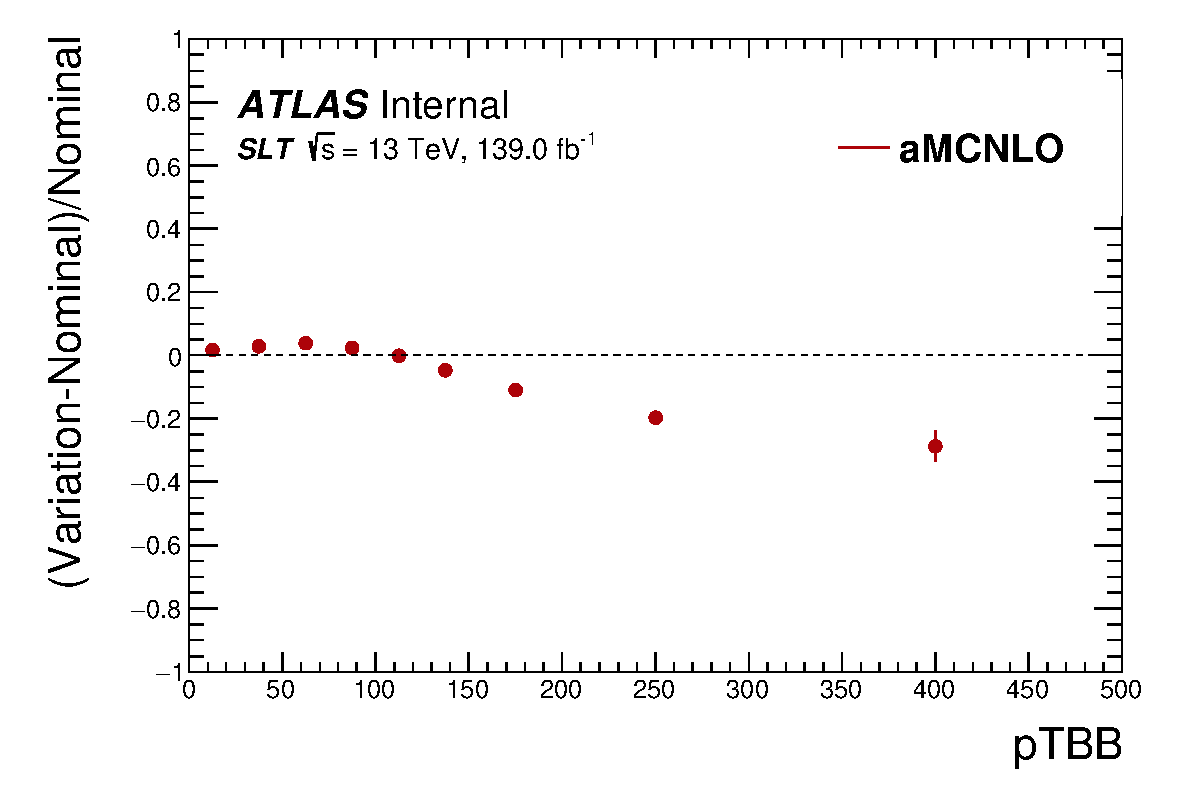
\includegraphics[width=.49\textwidth]{figures/lephad_modelling_systs/SLT/aMCNLO/pTBB_Norm.pdf}}
\subfloat[b]{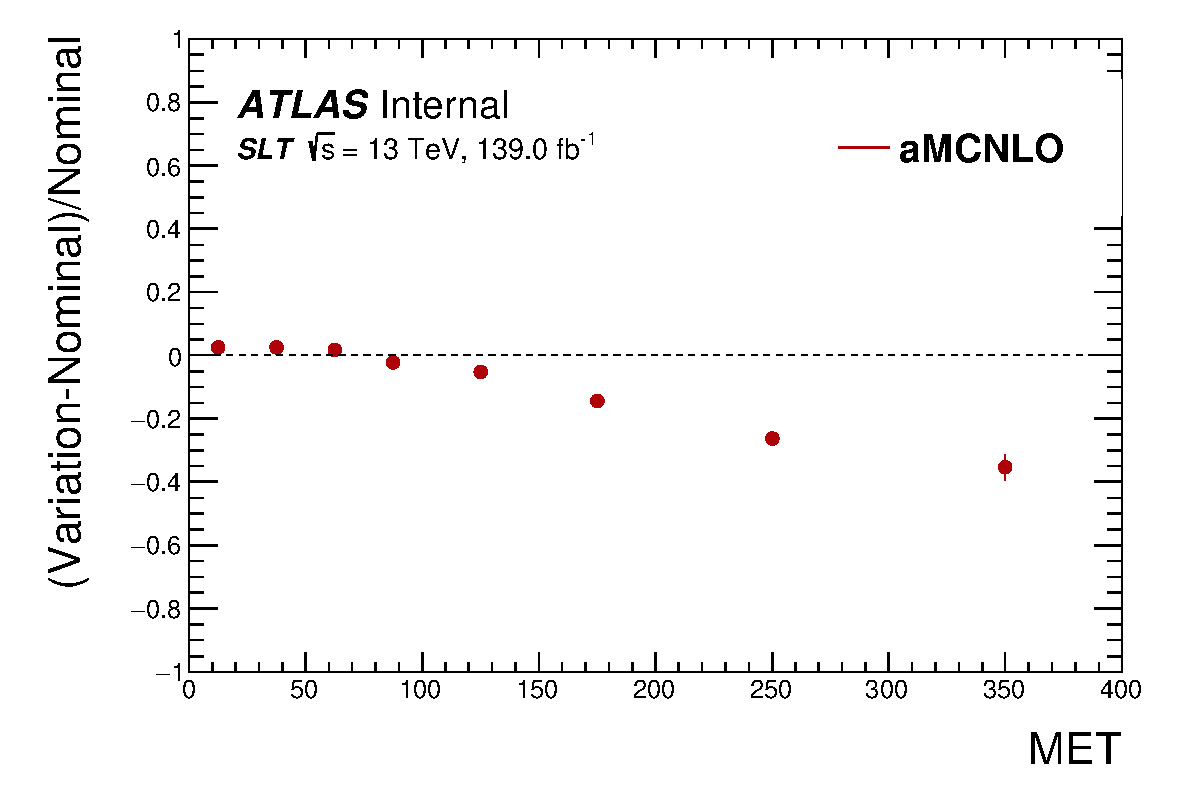
\includegraphics[width=.49\textwidth]{figures/lephad_modelling_systs/SLT/aMCNLO/MET_Norm.pdf}}
\caption{The shape-only parametrisation in bins of $p_T^{bb}$ (a) and in \met\ 
for the matrix element uncertainty, 
derived in the SLT channel.}
\label{fig:ttbarsyst_lephad_amc_SLT}
\end{figure}

The $p_T^{bb}$ and \met\ distributions are checked again for the 
weighted samples as compared to the variation samples. 
Good closure is found in both distributions and in other MVA discriminant
input variables. 
To check how well the weighted nominal sample can recover the MVA output distributions
of the variation sample, the NN score distribution of the variation 
and the weighted nominal is shown in Figure~\ref{fig:ttbarsyst_lephad_amc_NN},
where the events yields of the variation sample are 
normalised to the ones of the nominal.

% and more plots showing the closure in the PNN scores are in
%  Appendix~\ref{subsec:appendix_systs_ttbarsysts_lephad}.
\begin{figure}
\centering
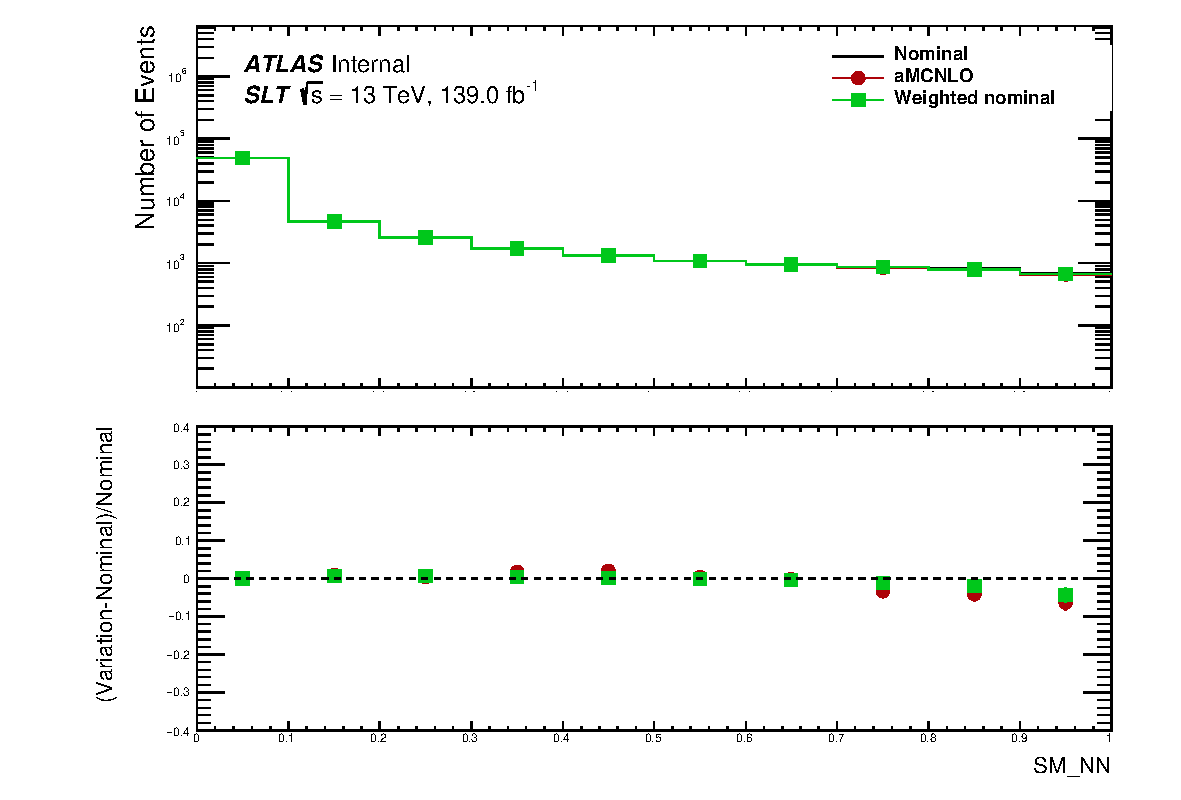
\includegraphics[width=.49\textwidth]{ figures/lephad_modelling_systs/SLT/aMCNLO/Hist_and_ratio_SM_NN_Norm.pdf}
\caption{SLT channel: shape-only NN score of the matrix element variation sample and the weighted nominal, using sequential parametrisation
in $p_T^{bb}$ and \met.
The binning shown here is in euqal width bins of NN score. }
\label{fig:ttbarsyst_lephad_amc_NN}
\end{figure}
  
The parton shower uncertainty is first checked with 
parametrisation in single MVA variable
but none of the MVA discriminant input alone give good closure in the MVA output distributions. 
Therefore, a similar sequential parametrisation approach is used.
The parametrisation is done first 
in bins of the \pt\ of the subleading jet ($p_T^{b2}$) 
followed by parametrising the residue in bins
of mass of the di-Higgs system ($m_{HH}$), 
as shown in Figure~\ref{fig:ttbarsyst_lephad_herwig}.
The closure of the parametrisation in the NN score is shown in 
Figure~\ref{fig:ttbarsyst_lephad_herwig_NN}.
\begin{figure}
\subfloat[a]{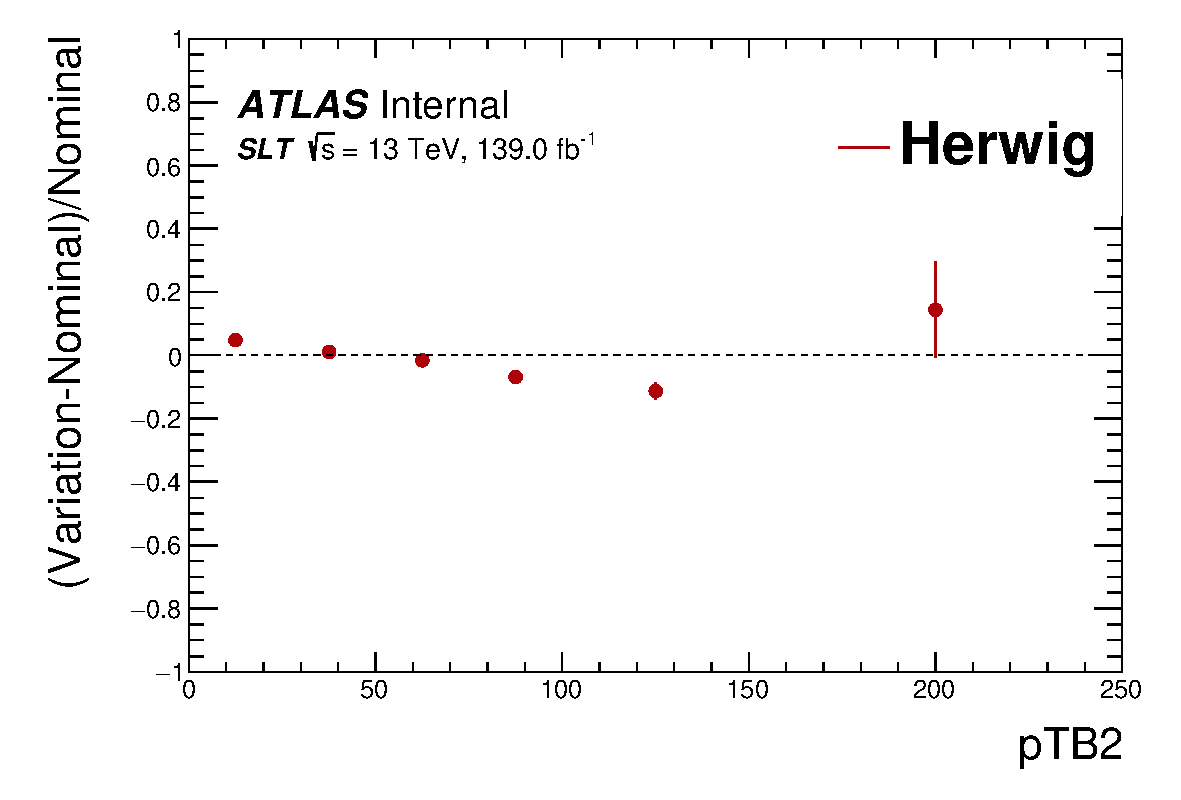
\includegraphics[width=.49\textwidth]{figures/lephad_modelling_systs/SLT/Herwig/pTB2_Norm.pdf}}
\subfloat[b]{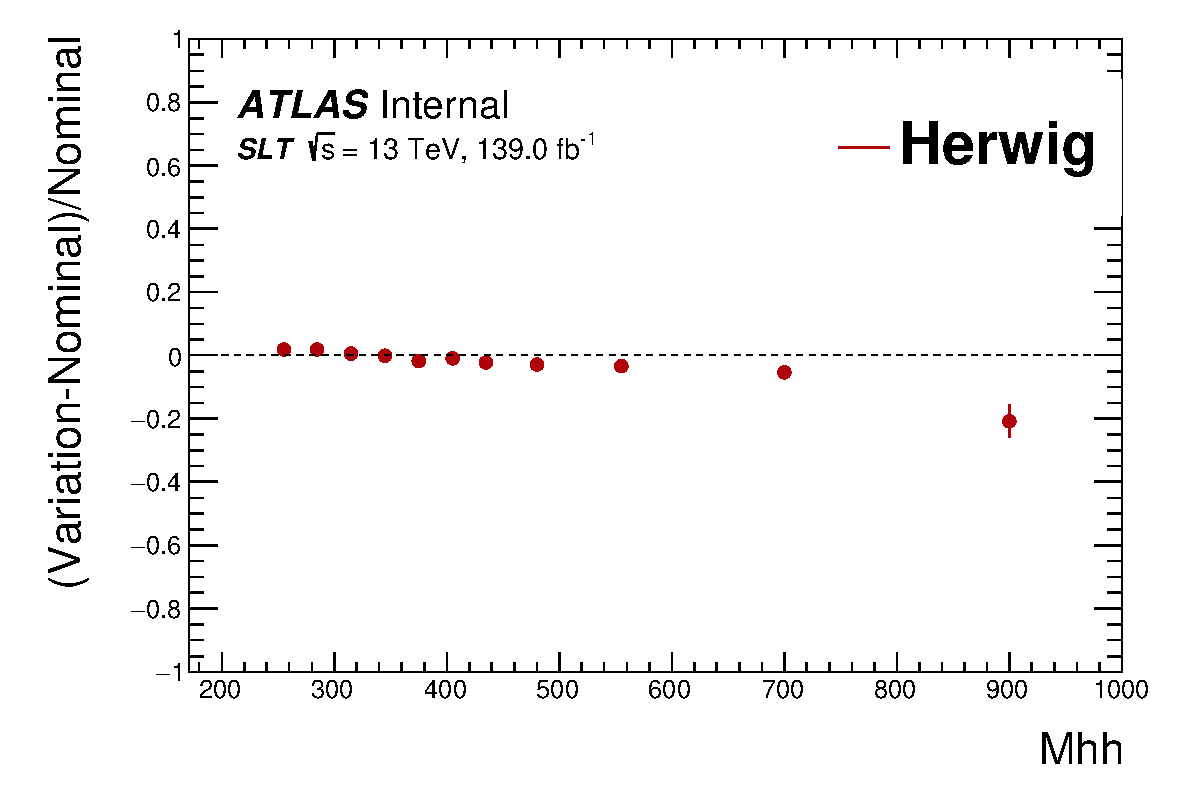
\includegraphics[width=.49\textwidth]{figures/lephad_modelling_systs/SLT/Herwig/Mhh_Norm.pdf}}
\caption{The shape-only parametrisation in bins of $p_T^{b2}$ (a)
in $m_{HH}$ (b), for the parton shower uncertainty, derived in the 
SLT channel.}
\label{fig:ttbarsyst_lephad_herwig}
\end{figure}

\begin{figure}
\centering
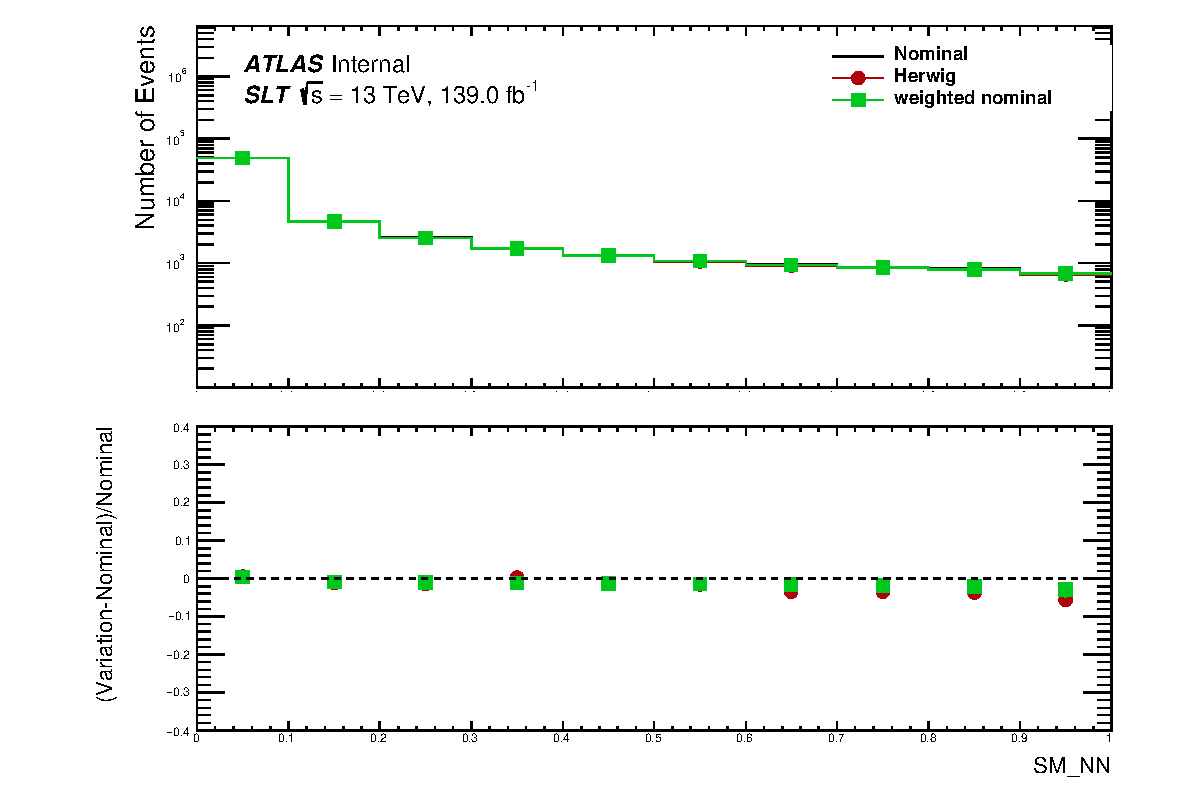
\includegraphics[width=.49\textwidth]{figures/lephad_modelling_systs/SLT/Herwig/Hist_and_ratio_SM_NN_Norm.pdf}
\caption{The shape-only NN score of the parton shower variation sample and the weighted nominal.
The binning shown here is in euqal width bins of NN score. }
\label{fig:ttbarsyst_lephad_herwig_NN}
\end{figure}


The sequential parametrisation method is compared with
the second method, which is based on  
parametrising directly in the ratio of MVA discriminant output of the variation samples to the 
ones of the nominal. 
The binning used for parametrisation is the same as the binning used in the final fit. 
Due to the very fine binning in the high MVA output region, 
large statistical fluctuations is observed, therefore,
smoothing is applied on these systematics in limit setting to reduce the fluctuations effect. 
The SM NN parametrisation for the matrix element and parton shower variation in the SLT channel is shown in 
Figure~\ref{fig:ttbarsyst_lephad_SLT_NN}.
Plots for more resonant mass points can be found in Appendix~\ref{sec:appendix:systs}.

\begin{figure}
\centering
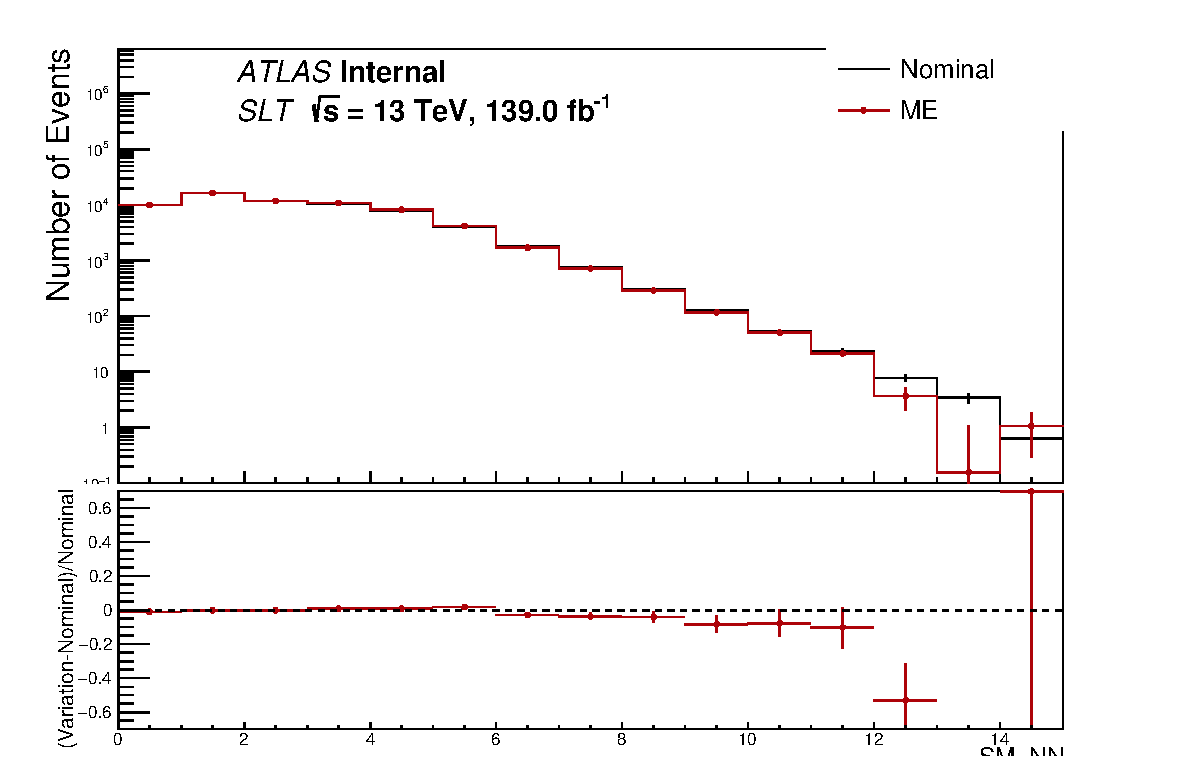
\includegraphics[width=.49\textwidth]{figures/lephad_modelling_systs/SLT/ME/limit_binning_SM_NN_Norm}
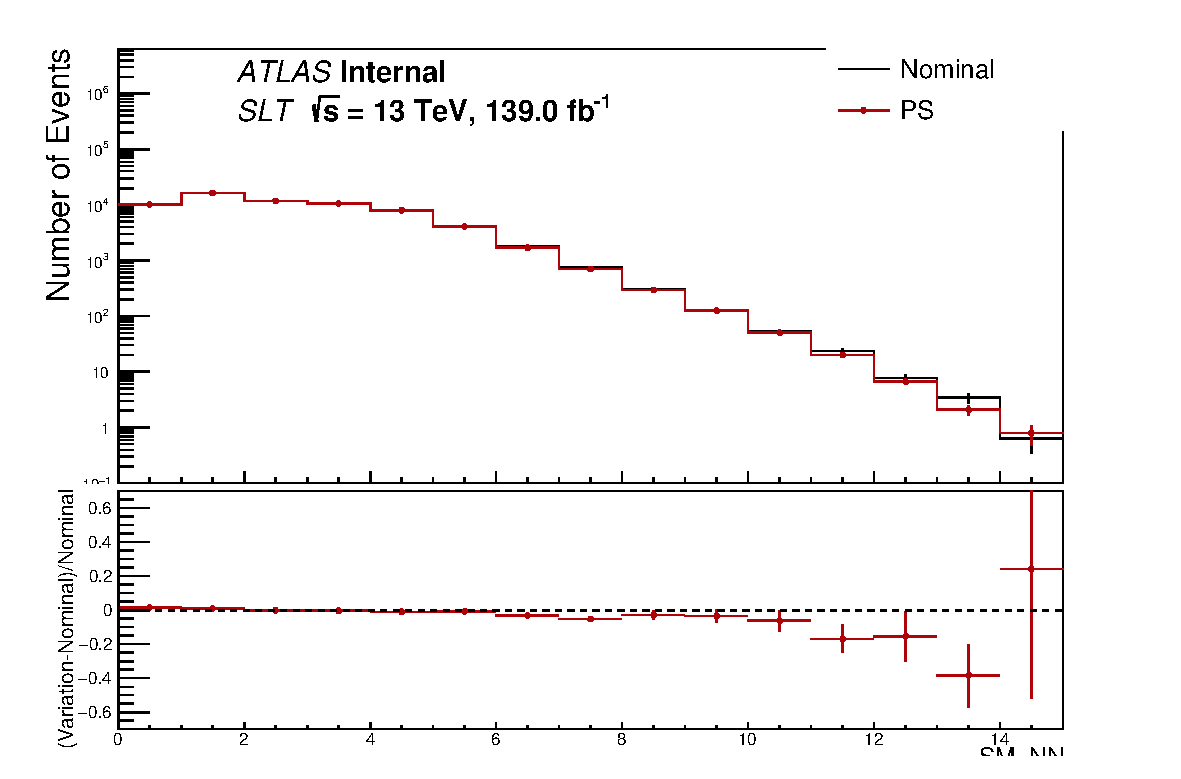
\includegraphics[width=.49\textwidth]{figures/lephad_modelling_systs/SLT/PS/limit_binning_SM_NN_Norm}\\
% 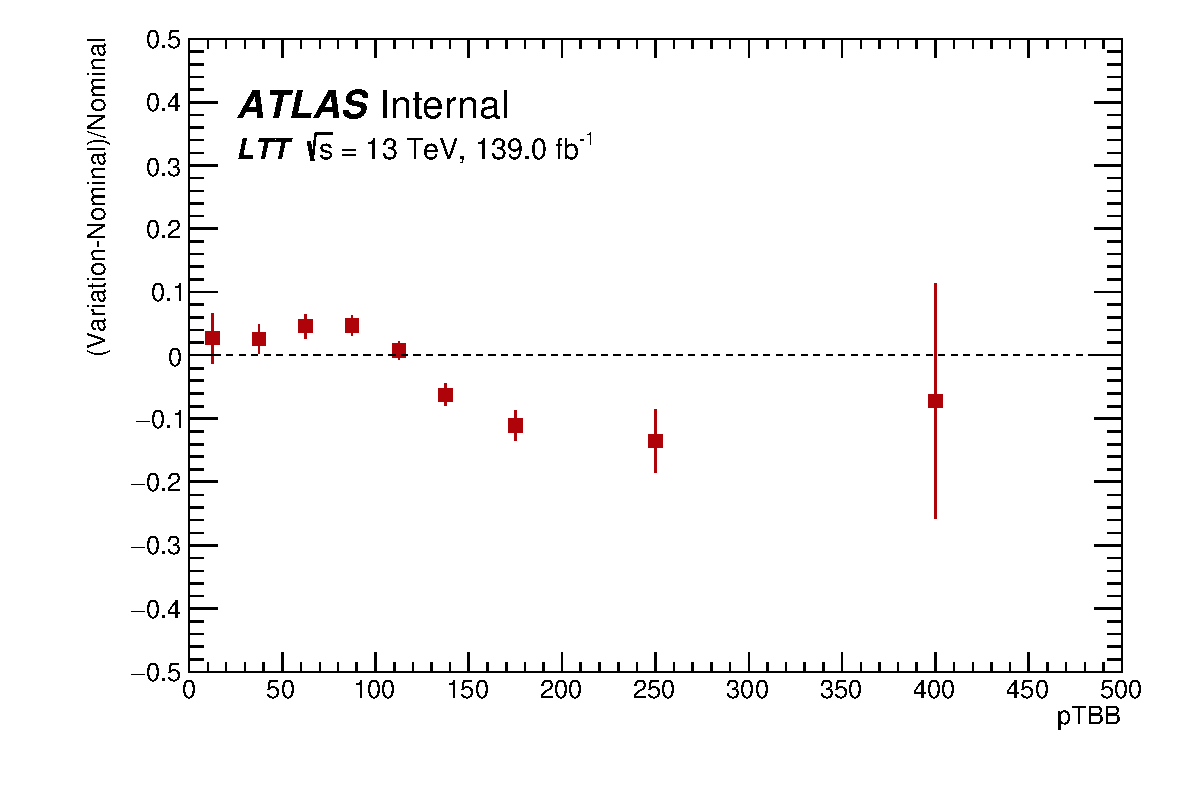
\includegraphics[width=.49\textwidth]{figures/lephad_modelling_systs/LTT/aMCNLO/pTBB_Norm}
% 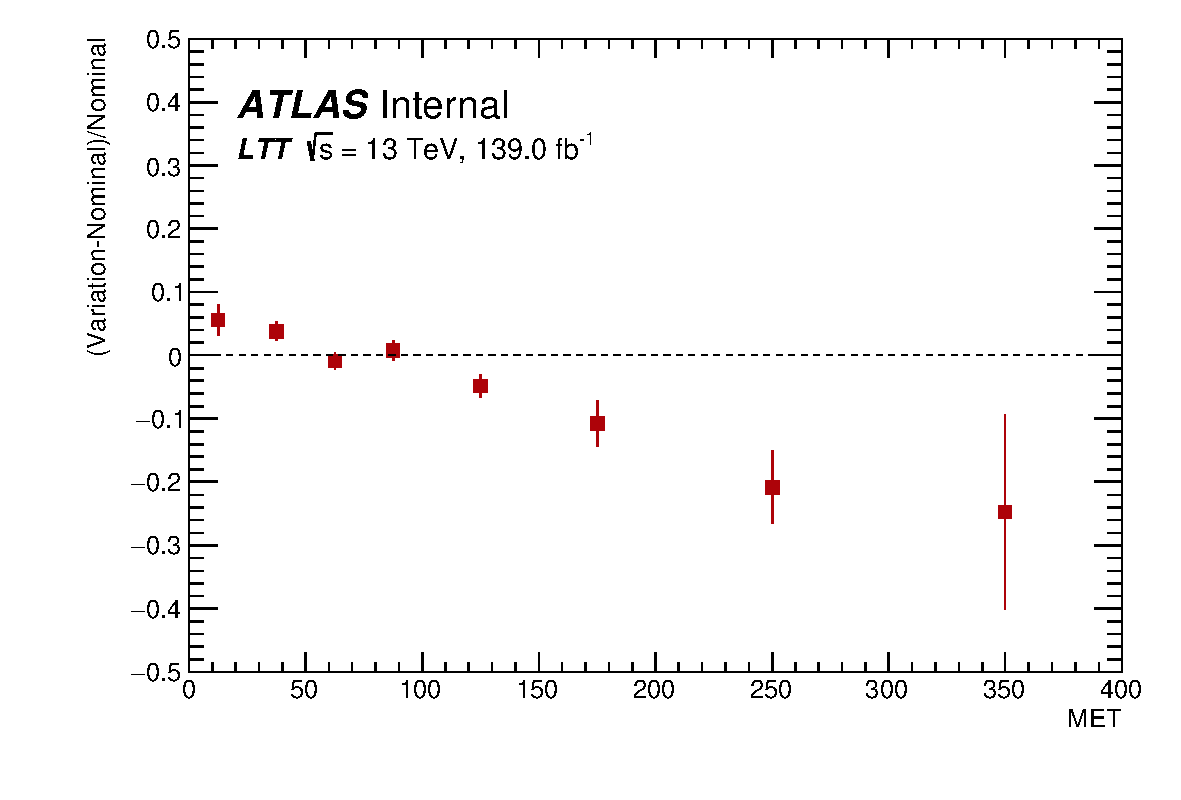
\includegraphics[width=.49\textwidth]{figures/lephad_modelling_systs/LTT/aMCNLO/MET_Norm}
\caption{Parametrisation in SM NN score distribution for the ME (left) and PS (right) systematics.
The binning is the same as the final fit binning.}
\label{fig:ttbarsyst_lephad_SLT_NN}
\end{figure}


The main reason for using the second method is to ease the combination to
the other channels, and to reduce complexity, eventhough the second method has some drawbacks. 
Also in the high MVA score region,
where the binning becomes much finer, the first method starts to fail to cover 
the large difference between the variation and the nominal samples.


The ISR up and down variations have not shown obvious shape 
in the NN/PNN distribution therefore only normalisation uncertainty is considered. 


\paragraph{Uncertainties on $t\bar{t}$ in the \ZHF\ control region}\mbox{}\\

Shape uncertainties on the $t\bar{t}$ background are neglected in the \ZHF\ 
control region as they are found to be negligible 
in the $m_{\ell\ell}$ distribution included in the 
fit for this region, as shown in Figure~\ref{fig:append:ZHFttbar} in 
Appedix~\ref{sec:appendix:systs}.





\subsubsection{Uncertainties on \texorpdfstring{\ZHF}{Z+HF}\ background}
\label{sec:DiHiggs:ZHFsysts}
The normalisation of the \ZHF\ background is estimated 
from data as included as freely floating parameter in 
the final fit. This normalisation is mainly determined 
from the dedicated \ZHF\ dilepton control region.
% All these uncertainties are derived by MC-to-MC comparison, 
% as described in Section~\ref{sec:systematics_backgroundmodelling}, 
% following the \href{https://twiki.cern.ch/twiki/bin/viewauth/AtlasProtected/PmgWeakBosonProcesses}{\underline{recommendations of the PMG group for Weak Boson processes}}. 
Only \ZHF\ background are considered, 
including $Z+bb$, $Z+bc$, $Z+cc$. 
Contributions from Z + light flavour jets 
such as $Z$+light jets($Z+l$), $Z+bl$ and $Z+cl$ are excluded. 

Uncertainties due to choice of matrix element generators are evaluated
by comparing the \textsc{Sherpa}~2.2.1 samples to the
\MADGRAPH+\textsc{Pythia}~8 samples. 
Uncertainties on the $Z$+jets background modelling 
related to the choice of renormalisation and factorisation 
scales are evaluated using event weights included 
in the \textsc{Sherpa}~2.2.1 samples, varying the scales either together 
or independently up and down by a factor of two, 
leading to 7-point scale variations. 
% The scale uncertainty is then given by the maximum shift 
% of the envelope with respect to the nominal, from which 
% the envelope around the nominal can be worked out. 
The uncertainty due to the choice of PDF set is evaluated 
by comparing the \texttt{NNPDF3.0} PDF set to two other PDF sets,
to two \texttt{NNPDF3.0} PDF varied $\alpha_s$ values. 
The difference between these PDF sets are covered in an envelope and 
the envelope is taken to be the intra-PDF uncertainty. 
The inter-PDF set uncertainty is estimated by 
calculating the standard deviation of 101 replicas of
\texttt{NNPDF3.0} PDF set. 

% in a similar way, using the event weights included in the samples. 
% The PDF variations include 100 replicas of the nominal \texttt{NNPDF3.0} PDF set 
% as well as central values for two different PDF set, 
% \mmhtnnlo\ and \ctfourteennlo, and two \nnpdfnnlo\ $\alpha_s$ variations.  
% The NNPDF intra-PDF uncertainty is estimated as the standard deviation 
% of the set of 101 \texttt{NNPDF3.0} sets. 
% The envelope of the differences between the nominal NNPDF set 
% and the other two PDF sets is taken as an additional uncertainty. 

From the nominal Sherpa configuration there are two other parameters 
that can be varied to introduce uncertainties 
on the modelling of the $W$/$Z$+jets process: 
matrix element matching (\textit{ckkw}), which varies the scale taken 
for the calculation for the overlap between jets 
from the matrix element and the parton shower. 
The nominal value for this parameter is 20~GeV. 
The up variation increases this to 30~GeV, 
while the down variation decreases the nominal value to 15~GeV. 
The second parameter is the resummation scale (\textit{qsf}), 
which varies the scale used for the resummation 
of soft gluon emission $\mu_{qsf}$ is varied from 2 and with respect to the nominal. 

Relative acceptance normalisation uncertainties between the CR and the SR are calculated 
from the single channel acceptances using Equation~\ref{eq:relative_acceptance_unc} 
as reported in Table~\ref{sec:systs:tab:systematics_normalisations_ZHF}.


\begin{table}
\centering
\small
\begin{tabular}{|c|c|c|}
\hline
Source & SLT & LTT\\
\hline
ME & +0.021, -0.021 & +0.10, -0.10 \\
Scales & -0.029, +0.053 & -0.054, +0.085 \\
CKKW & +0.07, -0.07 &  +0.071, -0.071 \\
QSF & -0.016, +0.016 & -0.016 , +0.016 \\
PDF+$\alpha_s$ & -0.0026, +0.0026 & -0.0033 , +0.0033 \\
PDF choice & -0.0097, +0.0097 & -0.011, +0.011 \\
Total & -0.081, +0.092 & -0.14, +0.15 \\
\hline
\end{tabular}
\caption{Relative size of relative acceptance normalisation uncertainties on \ZHF\ for the di-Higgs analysis.}
\label{sec:systs:tab:systematics_normalisations_ZHF}
\end{table}




For the 7-point scale variation, the ratios of the normalised MVA output distributions of the varations
to the one of the nominal are checked. Obvious shape is observed, and
a similar parametrisation approach is used.
All MVA discriminant input variables were considered for the parametrisation. 
Instead of parametrising all seven points of variation, the parametrisation is considered
for the envelope encapsulating the maximum shift of the variation. 
The variable to parametrise is chosen such that the 
weighted nominal samples can best recover the envelop covering the maximum shift in the PNN scores. 
As a result, the envelope is parametrised by the $p_T^{bb}$,
as shown in Figure~\ref{fig:lephad_ZHF_scale_pTBB}.
In the figure, the weighted nominal samples distributions 
are labelled as `para:pTBB Up(Down)' and the maximum shift of the 7-point variations in the MVA
output distributions are covered by the envelope labelled as `Envelop\_Up(Down)'. 


\begin{figure}[htbp]
\centering
\subfloat[]{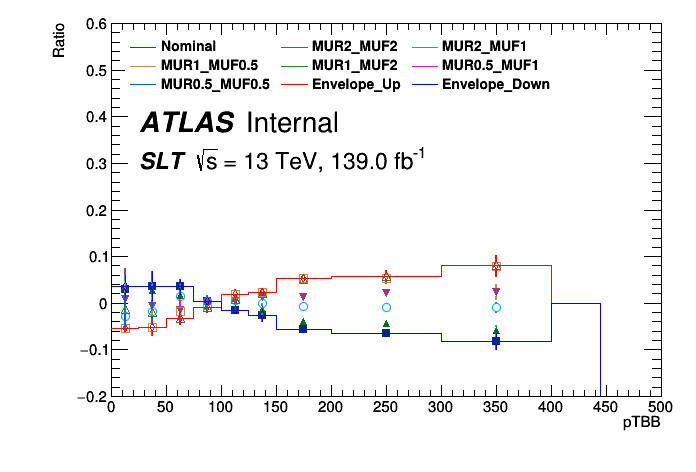
\includegraphics[width=.41\textwidth]{figures/lephad_modelling_systs/SLT/ZHF_scale/Ratio_pTBB_Norm.png}}\quad
\subfloat[]{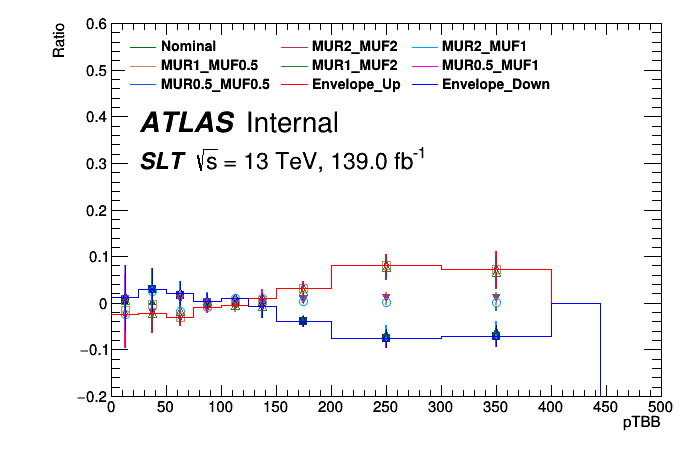
\includegraphics[width=.41\textwidth]{figures/lephad_modelling_systs/LTT/ZHF_scale/Ratio_pTBB_Norm.png}}\quad
\caption{SLT (left) and LTT channel (right): Taking an envelope of the \ZHF\ scale variation with $p_T$ of the 2 $b$-jets.}
\label{fig:lephad_ZHF_scale_pTBB}
\end{figure}
    
the PNN score distribution is shown in Fig.\ref{fig:lephad_ZHF_scale_SLT_PNN} 
for the SLT channel and Fig.\ref{fig:lephad_ZHF_scale_LTT_PNN} for the LTT channel.
Good closure within statistical uncertainty is observed using this parametrisation.


\begin{figure}
\centering
\subfloat[]
    {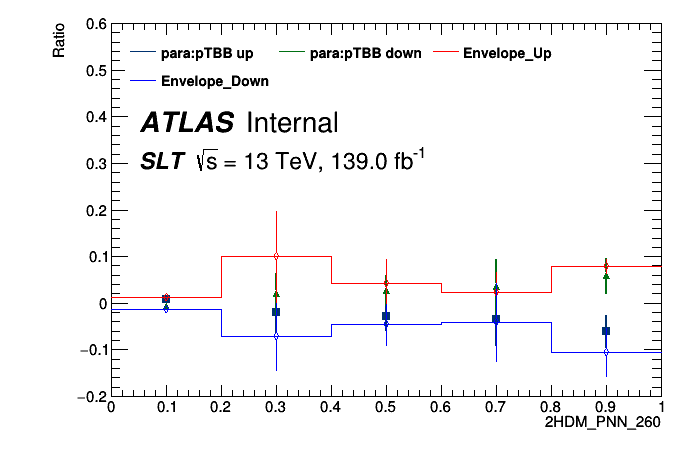
\includegraphics[width=.41\textwidth]{figures/lephad_modelling_systs/SLT/ZHF_scale/Ratio_2HDM_PNN_260_Norm.png}} \quad
\subfloat[]
    {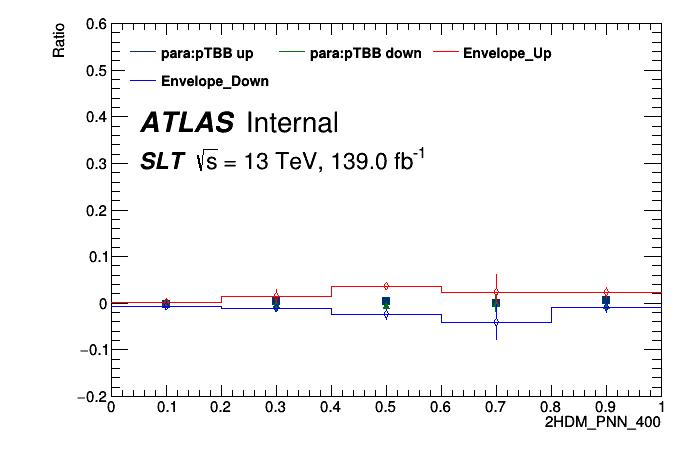
\includegraphics[width=.41\textwidth]{figures/lephad_modelling_systs/SLT/ZHF_scale/Ratio_2HDM_PNN_400_Norm.png}} \quad
\subfloat[]
    {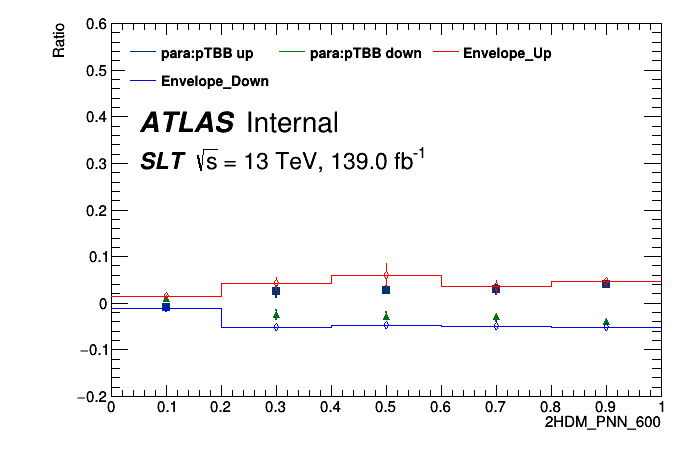
\includegraphics[width=.41\textwidth]{figures/lephad_modelling_systs/SLT/ZHF_scale/Ratio_2HDM_PNN_600_Norm.png}} \quad
\subfloat[]
    {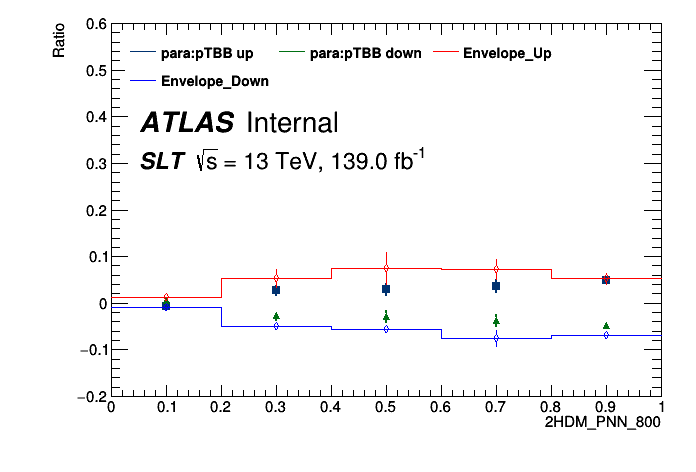
\includegraphics[width=.41\textwidth]{figures/lephad_modelling_systs/SLT/ZHF_scale/Ratio_2HDM_PNN_800_Norm.png}} \quad
\caption{SLT channel: PNN output distributions of the nominal sample weighted by parametrisation in 
$p_T^{bb}$, labelled as `para:pTBB Up(Down)' versus envelope encapsulating the maximum shift of the variation
for various resonant mass.}
\label{fig:lephad_ZHF_scale_SLT_PNN}
\end{figure}

    
    

\begin{figure}
\centering
\subfloat[]
{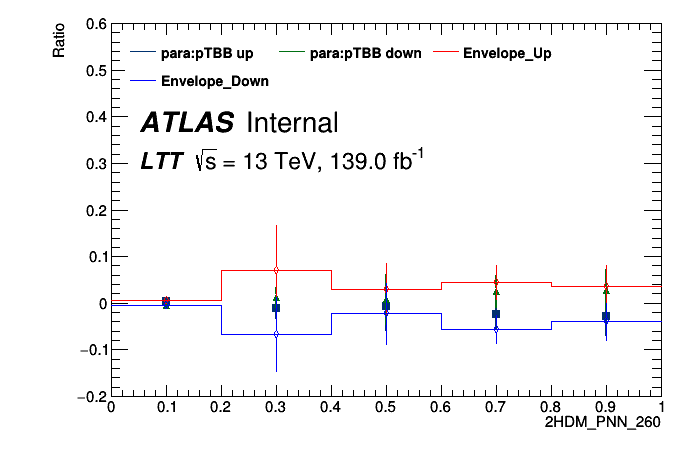
\includegraphics[width=.41\textwidth]{figures/lephad_modelling_systs/LTT/ZHF_scale/Ratio_2HDM_PNN_260_Norm.png}} \quad
\subfloat[]
{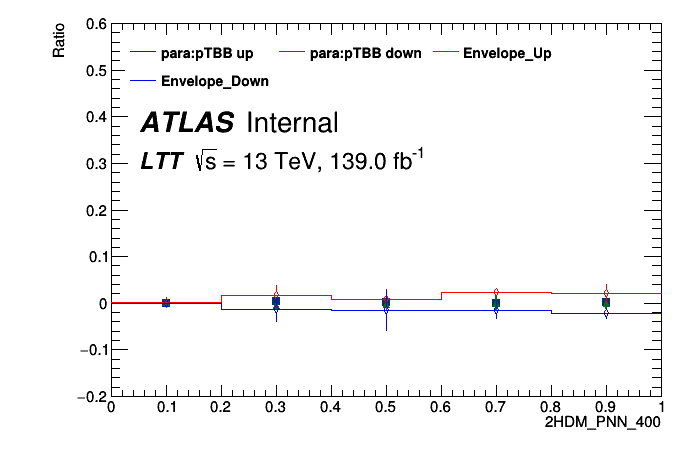
\includegraphics[width=.41\textwidth]{figures/lephad_modelling_systs/LTT/ZHF_scale/Ratio_2HDM_PNN_400_Norm.png}} \quad
\subfloat[]
{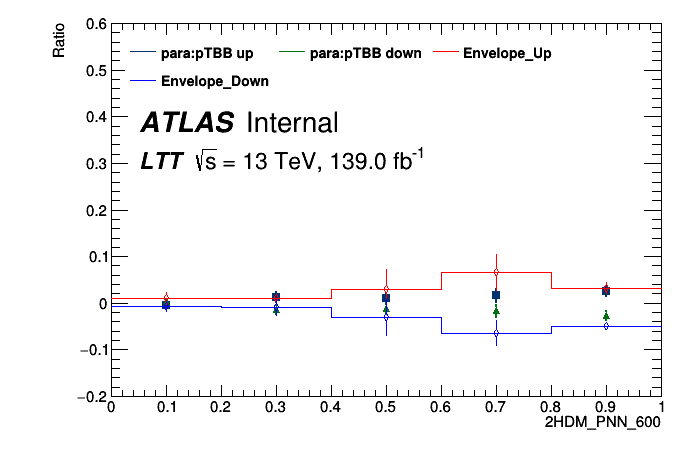
\includegraphics[width=.41\textwidth]{figures/lephad_modelling_systs/LTT/ZHF_scale/Ratio_2HDM_PNN_600_Norm.png}} \quad
\subfloat[]
{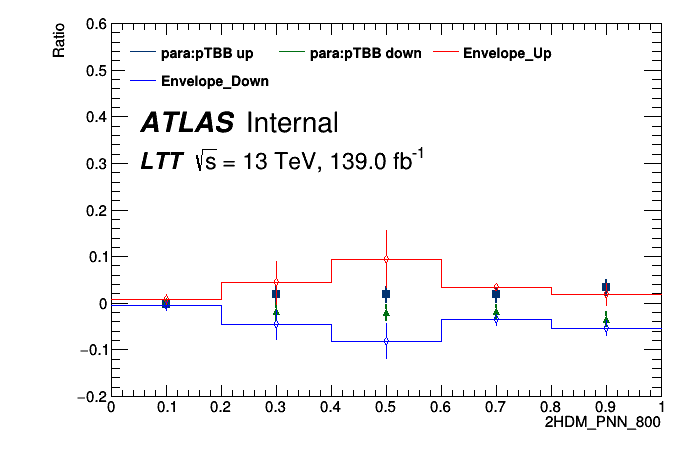
\includegraphics[width=.41\textwidth]{figures/lephad_modelling_systs/LTT/ZHF_scale/Ratio_2HDM_PNN_800_Norm.png}} \quad
\caption{LTT channel: PNN output distributions of the nominal sample weighted by parametrisation in 
$p_T^{bb}$, labelled as `para:pTBB Up(Down)' versus envelope encapsulating the maximum shift of the variation
for various resonant mass.}
\label{fig:lephad_ZHF_scale_LTT_PNN}
\end{figure}
    

For the uncertainty due to generator variation, 
the ratios of the variance to the nominal are checked in the MVA output. 
For most of the bins and mass points, no significant deviation from unity is observed
within the statistical uncertainty.
Similarly, the shape dependence on the uncertainty due to choice of intra/inter-PDF set,
$\alpha_s$ variations, ckkw and qsf are checked. 
No obvious trend is observed. The normalised ratio of 
the PNN distribution of thevariation mentioned above to
the nominal are shown in Appendix~\ref{sec:appendix:systs}, 
in Figure~\ref{fig:lephad_ZHF_Madgraph_SLT_PNN} (\ref{fig:lephad_ZHF_Madgraph_LTT_PNN})
for the generator uncertainty, 
Figure~\ref{fig:lephad_ZHF_PDF_SLT_PNN} (\ref{fig:lephad_ZHF_PDF_LTT_PNN})
for the intra-PDF set uncertainties,
Figure~\ref{fig:lephad_ZHF_nnlo_SLT_PNN} (\ref{fig:lephad_ZHF_nnlo_LTT_PNN})
for the inter-PDF set and $\alpha_s$ uncertainty,
Figure~\ref{fig:lephad_ZHF_ckkw_SLT_PNN} (\ref{fig:lephad_ZHF_ckkw_LTT_PNN})
for the ckkw and qsf uncertainties in the SLT (LTT) channel.
The yields of the up and down variation for the ckkw and qsf 
uncertainties are both smaller than the nominal sample yields, 
and the solution for this issue is to normalize 
the central value of the up and down variation to the nominal sample, 
and take the difference from there. 

\paragraph{Uncertainties on \ZHF\ background in the \ZHF\ control region}\mbox{}\\

Shape uncertainties on the \ZHF\ background 
are neglected in the \ZHF\ control region as they are
found to be negligible in the $m_{\ell\ell}$ distribution included 
in the fit for this region, as shown in 
Appendix~\ref{sec:appendix:systs}.










\subsubsection{Uncertainties on single top}
\label{sec:DiHiggs:singletopsysts}
All single-top uncertainties are derived by MC-to-MC comparison,  
and split into the normalisation acceptance uncertainties and the 
shape uncertainties.


As the $W$t-channel contribution dominates over the $t$-channel and $s$-channel 
contributions, only the contribution from the $Wt$-channel is considered. 
Uncertainties due to PDF, ISR
and FSR are evaluated using internal alternative
weights present in all single-top nominal samples. 
Using the \texttt{PDF4LHC15\_30} PDF set, 
the uncertainties are estimated by combining the 
difference between the error sets and the nominal 
set following the recommendations in Ref.\cite{Butterworth:2015oua}.

Uncertainties from the parton shower, matrix element
and single top interference are estimated using 
the differences between the nominal samples and the corresponding 
alternative samples.
The parton shower uncertainty is evaluated comparing 
the AF2 nominal samples showered with \texttt{Pythia}~8 with alternative 
AF2 samples showered with \texttt{Herwig}~7.  
The matrix element uncertainty is evaluated comparing the AF2 nominal \POWHEG+\textsc{Pythia 8}
samples to the alternative AF2 \AMCatNLO+\textsc{Pythia 8} samples.  
Uncertainty due single-top interference is evaluated comparing the full simulated nominal 
\POWHEG+\textsc{Pythia 8} samples with diagram removal (DR) scheme to the alternative 
full simulation \POWHEG+\textsc{Pythia 8} sample with diagram subtraction (DS) scheme.

The normalisation acceptance uncertainties are shown in 
Table~\ref{sec:systs:tab:systematics_normalisations_singletop}.

\begin{table}
\centering
\small
\begin{tabular}{|c|c|c|}
\hline
Source & SLT & LTT \\
\hline
ME & -0.022, +0.022 & -0.15, +0.15  \\  
PS & +0.077, -0.077 & -0.093, +0.093  \\
Single top interference & +0.078, -0.078 & +0.11, -0.11  \\
ISR & -0.047, +0.064 & -0.045, +0.062  \\ 
FSR & -0.054, +0.043 & -0.069, +0.035,  \\
PDF & -0.032, +0.032 & -0.032, +0.032   \\
Total & $\pm 13.7\%$ & $\pm 21.1\%$ \\
\hline
\end{tabular}
\caption{Size of normalisation acceptance uncertainties for single-top background for the $HH$ analysis.}
\label{sec:systs:tab:systematics_normalisations_singletop}
\end{table}

  
The shape uncertainty is derived separately for the SLT channel and the LTT channels. 
Only normalisation acceptance uncertainty is considered for the parton shower and matrix element uncertainties 
as no obvious shape is observed in the NN or the PNN scores,
as shown in Appendix~\ref{sec:appendix:systs} 
in Figure~\ref{fig:singletopsyst_lephad_herwig_PNN_SLT},~\ref{fig:singletopsyst_lephad_aMC_PNN_SLT}
in the SLT channel and 
in Figure~\ref{fig:singletopsyst_lephad_herwig_PNN_LTT},~\ref{fig:singletopsyst_lephad_aMC_PNN_LTT}
in the LTT channel
for the parton shower, matrix element uncertainties, respectively.

% The FSR, scale, ISR and $\alpha_s$ uncertainties are 
% implemented by the internal weights of the single top MC samples 
% therefore no parametrisation is needed. 

For the single-top interference uncertainty, the parametrisation 
is extracted from the ratio of the variation to the nominal fullsim samples
in bins of $p_T^{bb}$ where it shows the most obvious trend and largest shift from unity.
Other MVA discriminant input are also tested, but most of them either do not have an obvious shape
or the variation size is much smaller compared to the $p_T^{bb}$, and therefore cannot 
provide sufficient closure in the MVA output distributions. 
The parametrisation is shown in Figure~\ref{fig:singletopsyst_lephad_interference_pTBB} 
(a), (b) for the SLT and the LTT channels respectively.
\begin{figure}
\centering
\subfloat[a]{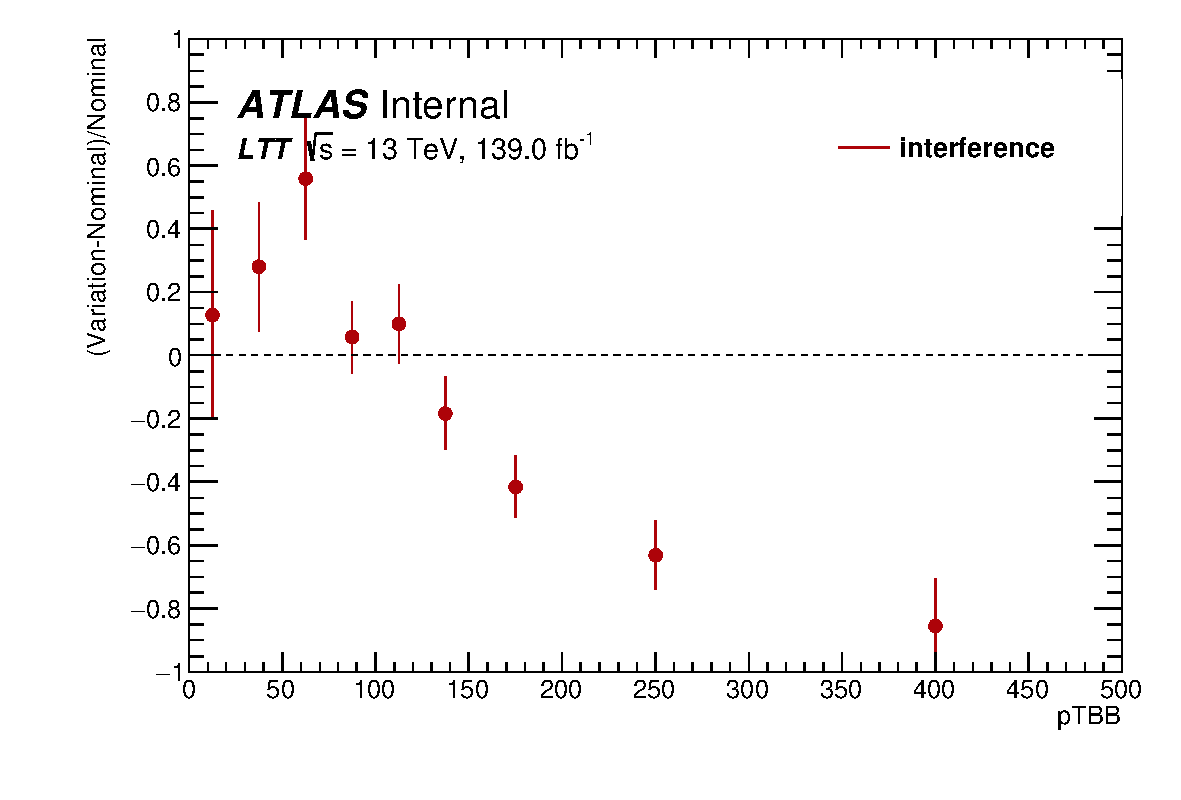
\includegraphics[width=.49\textwidth]{figures/lephad_modelling_systs/LTT/singletop/interference/pTBB_Norm}}
\subfloat[b]{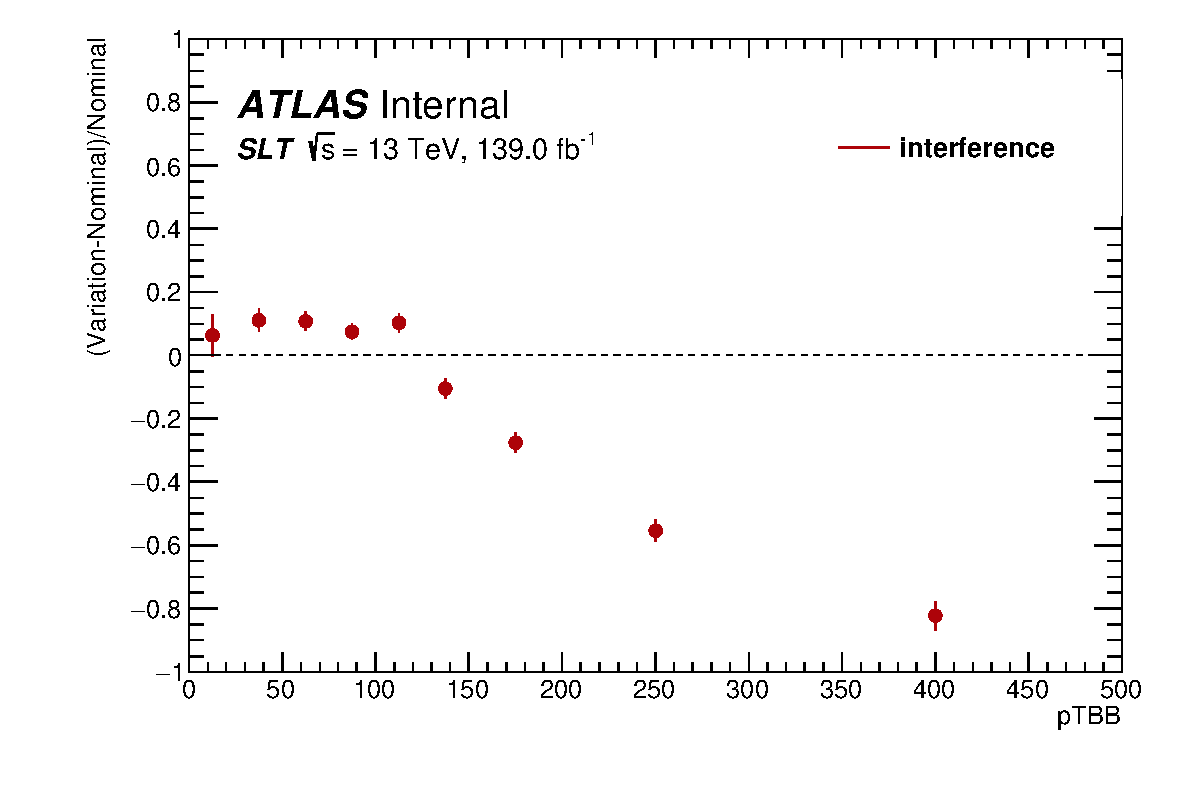
\includegraphics[width=.49\textwidth]{figures/lephad_modelling_systs/SLT/singletop/interference/pTBB_Norm}}
\caption{LTT (a) and SLT channels (b): shape only Parametrisation in bins of $p_T^{bb}$ distribution for $Wt$ DS/DR interference uncertainty.}
\label{fig:singletopsyst_lephad_interference_pTBB}
\end{figure}
The parametrisation is applied on the nominal sample as weights and the weighted sample
is passed through the MVA classification. 
The PNN score distributions of the weighted sample, and of the variation
sample are shown in Fig~\ref{fig:singletopsyst_lephad_interference_NN}. 
\begin{figure}
\centering
\subfloat[]{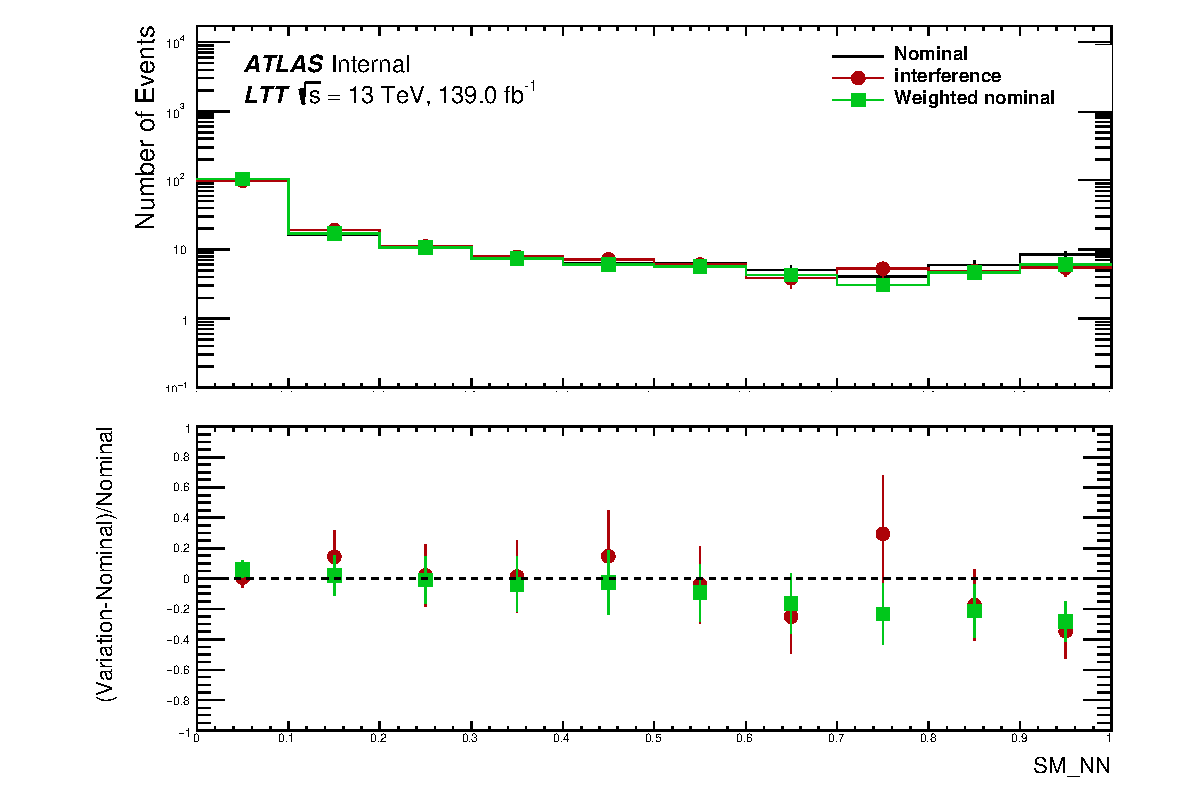
\includegraphics[width=.49\textwidth]{figures/lephad_modelling_systs/LTT/singletop/interference/Hist_and_ratio_SM_NN_Norm}}
\subfloat[]{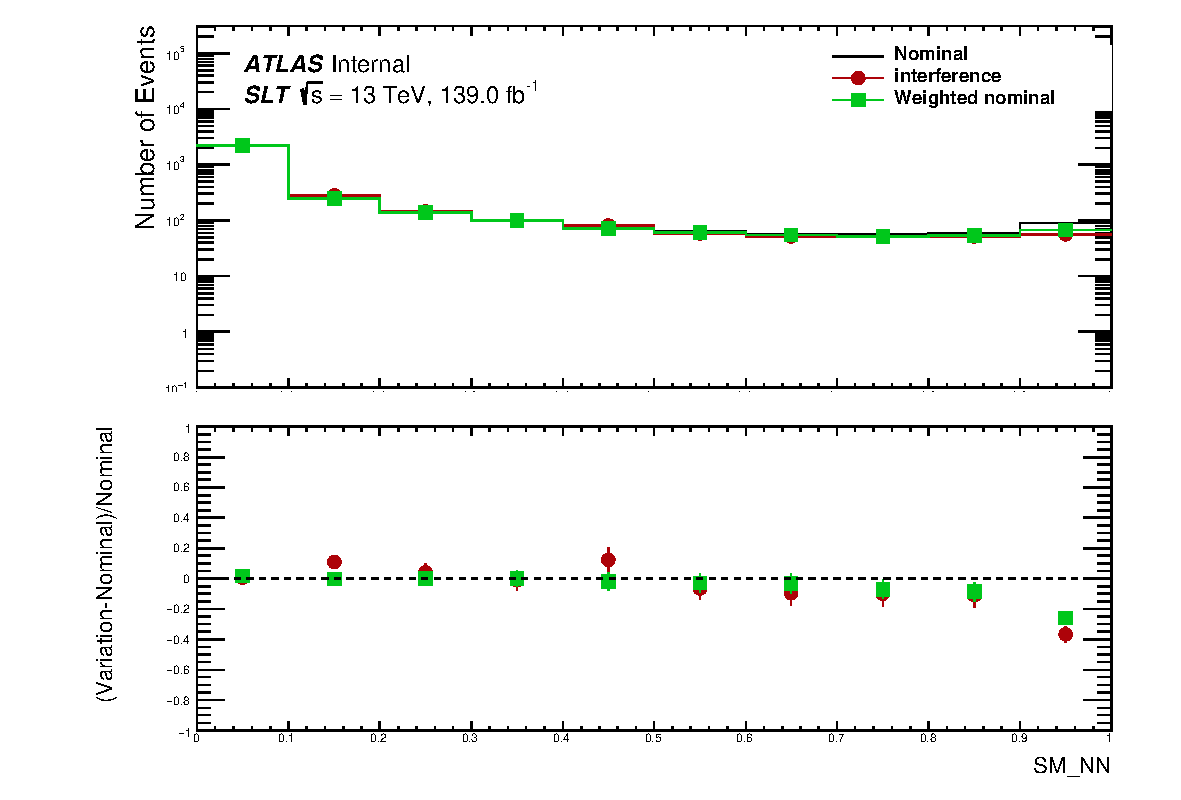
\includegraphics[width=.49\textwidth]{figures/lephad_modelling_systs/SLT/singletop/interference/Hist_and_ratio_SM_NN_Norm}}
\caption{LTT (left) and SLT channels (right): shape only SM NN score of the $Wt$ DS/DR interference uncertainty .}
\label{fig:singletopsyst_lephad_interference_NN}
\end{figure}    
The closure in the PNN scores for various resonance mass 
are shown in Appendix~\ref{sec:appendix:systs} in 
Figure~\ref{fig:singletopsyst_lephad_interference_PNN_SLT} 
and in Figure~\ref{fig:singletopsyst_lephad_interference_PNN_LTT}
for the SLT and LTT channels, respectively. 
Good closure is seen across various mass points of PNN classification
and in most of the bins, therefore the parametrisation in $p_T^{bb}$ is adopted.




\subsubsection{Uncertainties on single Higgs boson processes}
\label{sec:DiHiggs:singlehiggssysts}
Uncertainties on cross-section and BR are applied to all single Higgs boson 
processes included in the analysis as backgrounds 
(following recommendations from LHC Higgs Working Group~\cite{dihiggs-twiki}). 
% In addition to those, a 100\% uncertainty is applied on 
% the normalisation of the single Higgs boson processes without 
% real $b$-quarks (ggFHtautau, VBFHtautau and WHtautau) to 
% account for modelling of Higgs processes in association with extra 
% heavy flavor (conservative uncertainty motivated by 
% studies of heavy-flavour production in association with 
% top-quark pairs~\cite{PhysRevD.89.072012} and W boson production 
% in association with b-jets~\cite{Aad_2013} and from more 
% recent ttHyy studies~\cite{MorenoLlacer:2684286}, applied in all 
% di-Higgs analyses where relevant). No heavy-flavour uncertainty 
% is assigned to the ttH and ZH production modes, where the 
% dominant heavy-flavour contribution is already accounted for in the LO process.

For all single Higgs boson processes, uncertainties arised from PDF, 
$\alpha_s$ and scales are derived using 
internal alternative weights present in all the single Higgs boson nominal samples. 

For PDF and $\alpha_s$ variations, the 
\texttt{PDF4LHC\_NLO\_ 30} PDF set is used for evaluation.
The PDF set is comprised of of 30 eigenvectors parameterising 
the uncertainties for all the PDFs and 1 parameter for the $\alpha_s$ variations.
The variations of the PDF and \alphas\ are combined by 
taking the square root of the quadrature sum of the 30 eigenvectors variations
and the \alphas\ variation in bins of PNN score distributions.
The combined variation is then compared with the nominal \texttt{PDF4LHC\_NLO\_ 30} PDF
to evaluate the uncertainties due to PDF and \alphas.
The method used here follows the \texttt{PDF4LHC }
recommendations~\cite{Butterworth:2015oua}.

Variations of the renormalisation and factorisation scales
are used to estimate the uncertainty due to missing higher 
order corrections. For these scale variations, 
the 7-point scale variations of the renormalisation
and the factorisation scale are used and they are 
combined by taking an envelope of all of the variations,
similar to the method used in section~\ref{sec:DiHiggs:ZHFsysts}.
Parton shower uncertainties 
are evaluated comparing samples showered with \texttt{Pythia}~8
and \texttt{Herwig}~7 (with the matrix element provided by the same generator). 

For the ttH process,
the matrix element NLO matching uncertainty is evaluated 
comparing the nominal \POWHEG+\textsc{Pythia 8} samples 
to alternative \AMCatNLO+\textsc{Pythia 8} samples. 
Internal alternative weights are 
present in the nominal samples to evaluate the eigentune 
variations for ISR and FSR variations. 
The Var3c eigenvariation of the A14 tune, representing 
the variation of the strong coupling in the initial state shower, 
is used to evaluate the ISR uncertainty. 
The FSR uncertainty is evaluated using variations of $\mu_R$ 
by a factor 2 up and down around the nominal value in the parton shower. 

For the ZHbb process, the
ISR and FSR uncertainties are found to be negligible in the VHbb 
analysis as described in Ref~\cite{AlKhoury:2690042}, 
thus they are neglected in this analysis. 


The size of the acceptance uncertainties on the normalisations 
are reported in Table~\ref{sec:systs:tab:systematics_singleHiggs_AcceptanceNumbers}. 
Normalisation uncertainties smaller than 1\% are neglected in the analysis. 
After taking out the normalisation effects, 
shape effects were checked on the PNN score distributions 
and found to be negligible 
% as reported in Appendix~\ref{subsec:appendix_systs_singleHiggssysts} 
and therefore are not considered in the analysis.


\begin{table}
\centering
\small
\begin{tabular}{|c|c|c|c|}
\hline
Process   & SLT  & LTT  & Description\\
\hline
ttH  & -0.006,+0.006 & -0.008,+0.008   & PDF+$\alpha_s$ \\
ttH  & -0.003,+0.003 & -0.006,+0.006   & Scales\\
ttH  & -0.013,+0.013 & -0.067,+0.067  & PS\\
ttH  & -0.001,+0.001 & -0.01,+0.01  & ISR\\
ttH  & -0.051, +0.032 & -0.15, +0.055  & FSR\\
ttH  & -0.0025,+0.0025 & -0.019,+0.019  & ME NLO matching\\
ZHbb  & -0.006,+0.006 & -0.005,+0.005   & PDF+$\alpha_s$\\
ZHbb  & -0.030,+0.030 & -0.025,+0.025   & Scales\\
ZHbb  & -0.11,+0.11 & -0.037,+0.037   & PS\\
ZHtautau  & -0.0077,+0.0077 & -0.012,+0.012   & PDF+$\alpha_s$\\
ZHtautau  & -0.022,+0.022 & -0.028,+0.028   & Scales\\
ZHtautau  & -0.055,+0.055 & -0.15,+0.15   & PS\\
\hline
\end{tabular}
\caption{Relative size of single Higgs boson acceptance uncertainties in the di-Higgs analysis.
Table reproduced from analysis internal notes.}
\label{sec:systs:tab:systematics_singleHiggs_AcceptanceNumbers}
\end{table}



\subsubsection{Uncertainties on other minor backgrounds}
\label{subsec:uncertainties_minor_bkgs}

For minor backgrounds, i.e.\ single-top (s- and t-channels), 
Z+lf, W+jets and Diboson, acceptance uncertaintieas are 
only applied on the normalisation and their size is taken from the 
estimation performed in the SM VHbb analysis~\cite{ATLAS-CONF-2020-006, AlKhoury:2690042}.  
On single-top production an acceptance uncertainty of 20\% is applied  
in the s- and t-channels. 
An acceptance uncertainty of 23\% is applied on $Z$+lf. 
On W+jets an acceptance uncertainty of 37\% is applied 
in order to cover in addition for the fake-$\tau$ contribution 
(the uncertainty on the $\tau$-fakes in $W$+jets was estimated comparing 
the MC and the data-driven prediction for $W$+jets fakes in the 
0$b$-tag region of the \lephad channel to be 31\% in the previous iteration of this analsysis). 
Acceptance uncertainties of 25\%, 26\% and 20\% are applied on $WW$, $WZ$ and $ZZ$ respectively.








\subsection{Signal uncertainties}
\label{sec:systematics_signal}

Acceptance uncertainties on the resonant and non-resonant signals 
are evaluated by comparing the nominal signal samples to alternative 
MC samples for parton shower, PDF and scale variations.

\subsubsection{Resonant di-Higgs production}

The parton shower uncertainties for the resonant signals 
are estimated by comparing the nominal samples showered with 
\texttt{Herwig}~7 to alternative samples showered with \texttt{Pythia}~8 which are available 
in full-simulation for the $m_X= 500$ GeV and the $m_X=1000$ GeV mass points. 
The parton shower normalisation acceptance uncertainty is 
found to be 6\% (3\%) for $m_X=500$ ($m_X=1000$)~GeV 
in the SLT and 4\% (7\%) for $m_X= 500$ ($m_X=1000$)~GeV in the LTT. 
Thus, a conservative 6\% (7\%) uncertainty is adopted on the 
normalisation for all mass points in the SLT (LTT) channel.

After taking out the normalisation effect, the acceptance uncertainty on the 
shape of the PNN distribution is evaluated. 
Figure~\ref{fig:LepHadSLTSignalSysts} and \ref{fig:LepHadLTTSignalSysts} 
show the comparisons of the PNN distributions obtained from the 
nominal (black) and alternative (blue) signal samples for the  
$m_X= 500$ GeV and the $m_X=1000$ GeV mass points for the 
SLT and LTT SRs respectively. 
A linear fit to the ratio of the two distributions is 
performed to parameterise the shape variation as a function 
of the PNN score.
The linear function in the PNN score obtained from the fit 
performed at $m_X= 500$ GeV which has the largest slope, 
and this function is used to obtain the 
templates for the variations for all mass points. 
Relavant plots can be found in Appendix~\ref{sec:appendix:systs},
Figure~\ref{fig:LepHadSLTSignalSysts} and Figure~\ref{fig:LepHadLTTSignalSysts}. 

Scale, PDF and $\alpha_s$ uncertainties on signal are found to 
be negligible (less than 1\%) and therefore not included in the analysis. 

The resonant samples are generated with AF2 for masses up to 1 TeV (from \SI{1.1}{\TeV}
full simulation is used). Therefore the difference between the AF2 samples and
the full simulation samples is checked, using the 400~GeV mass point 
sample corresponding to 2017 and 2018 data-taking periods.  
The difference is less than 1\% in the SLT channel
and 2.9\% in the LTT channel, and there is no obvious shape
difference between the two types of simulation, as shown in
Figure~\ref{fig:Lephad_resonant_AF2_VS_FS}. 
The larger difference in acceptance times efficiency in 
LTT is originating from the \tauhad\ used in LTT triggers 
which no dedicated recommendations for AF2 exist.
Therefore a 3\% acceptance uncertainty is assigned to LTT of all signal
samples simulated with AF2 (up to 1~TeV mass point).

\begin{figure}
  \centering
  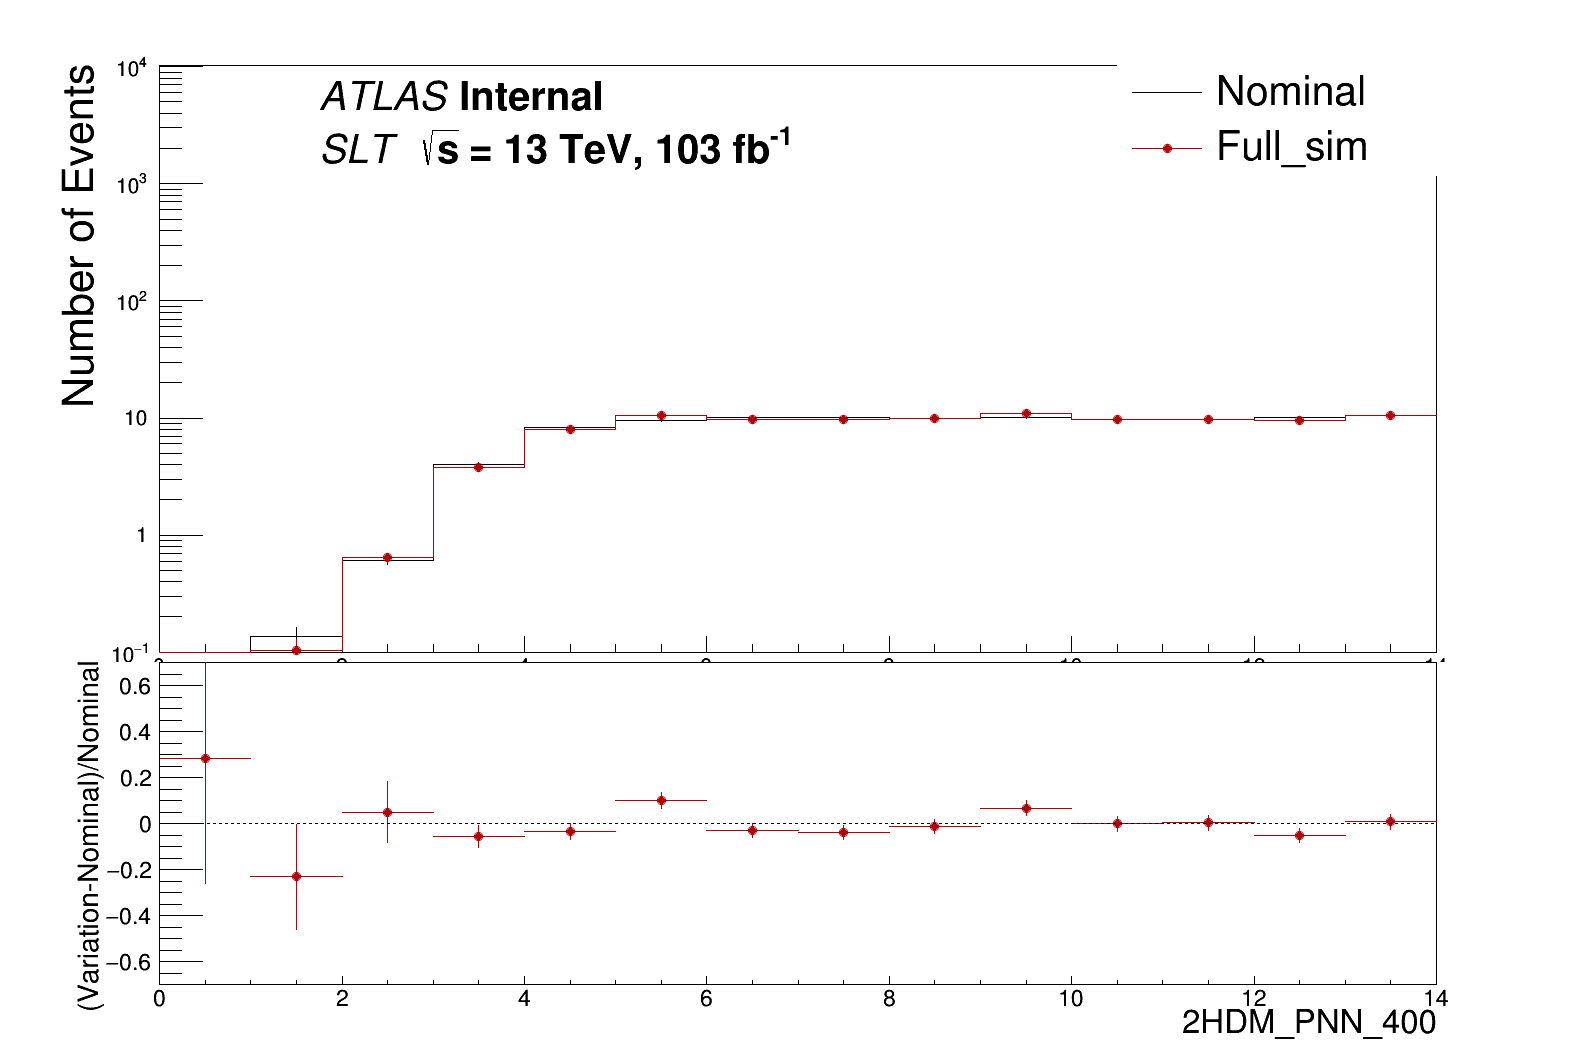
\includegraphics[width=.49\textwidth]{figures/lephad_modelling_systs/SLT/signal_AF2_check/limit_binning_2HDM_PNN_400_Norm.png}
  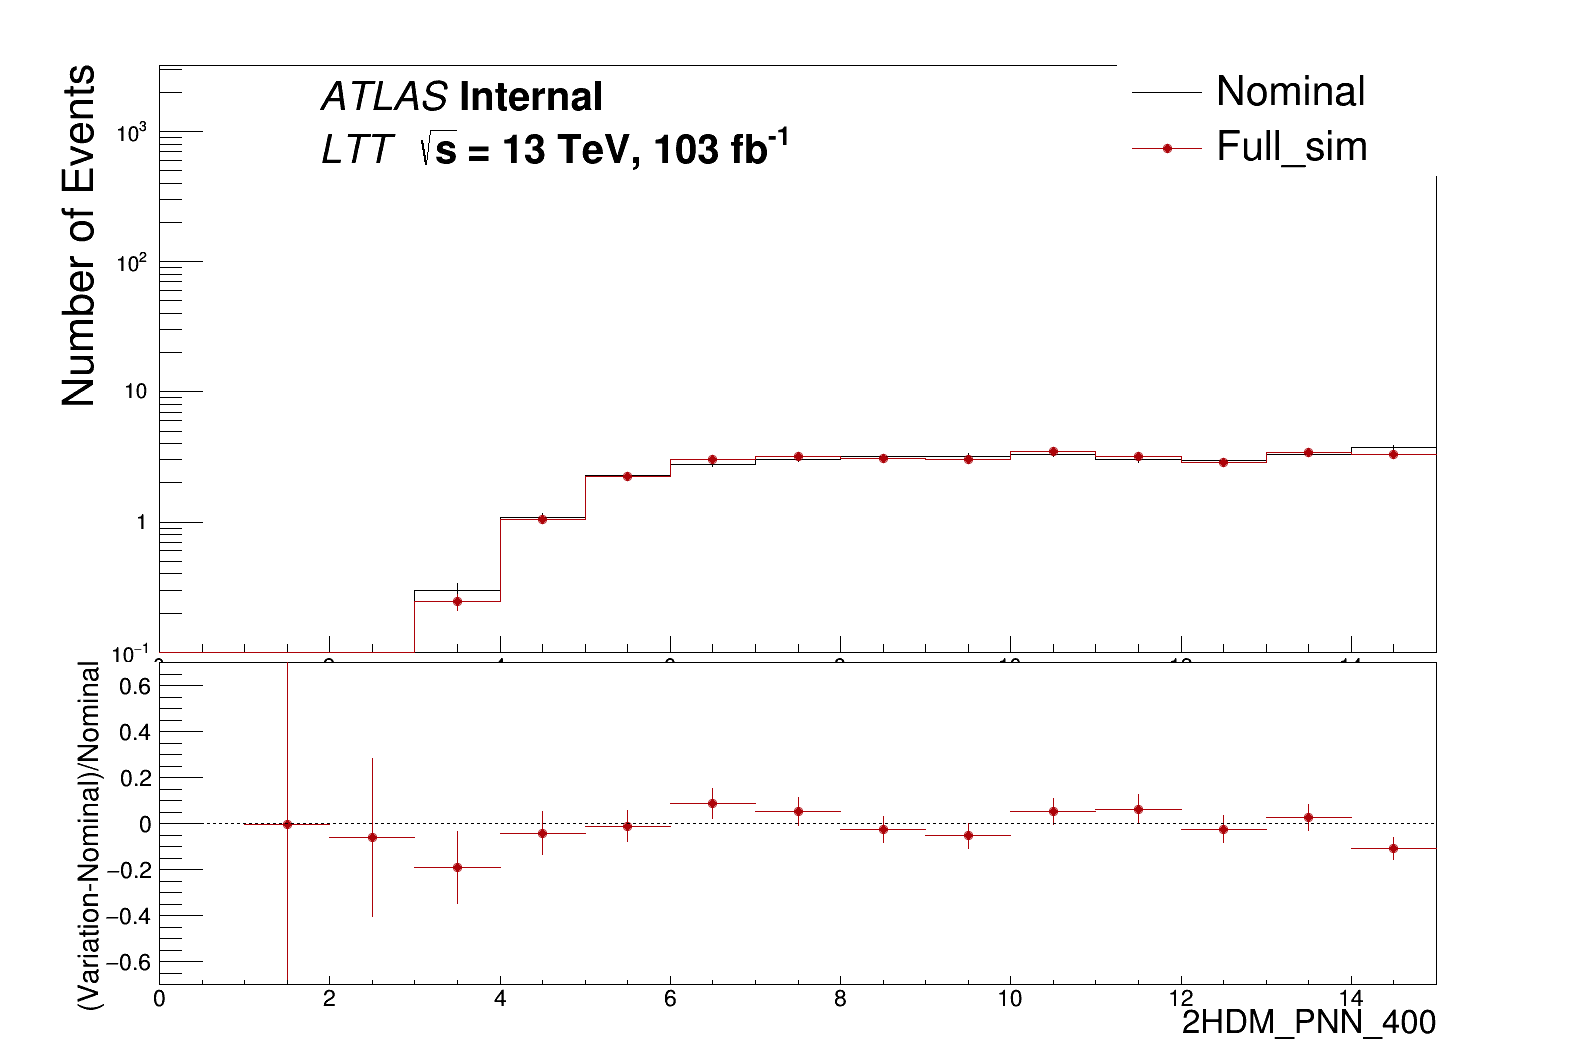
\includegraphics[width=.49\textwidth]{figures/lephad_modelling_systs/LTT/signal_AF2_check/limit_binning_2HDM_PNN_400_Norm.png}
  \caption{Comparison of the di-Higgs \lephad signal PNN distributions obtained from the nominal (AF2)
    and alternative (full simulation) signal samples for the  $m_X= 400$ GeV for the
    SLT (left) and the LTT (right) channel. The binning is the same as the final fit binning.
  }
  \label{fig:Lephad_resonant_AF2_VS_FS}
\end{figure}


All acceptance uncertainties on the signal normalisation obtained 
in the different signal regions are shown in 
Table~\ref{sec:systs:tab:systematics_HHSignal_AcceptanceNumbers}.  
\begin{table}
\centering
\small
\begin{tabular}{|c|c|c|c|}
\hline
Process X, GeV & SLT  & LTT & Description\\
\hline
$m_{X}= 400$  &  <0.01 & 0.029 & AF2\\
$m_{X}= 500$  &  0.06 & 0.05 & PS\\
$m_{X}= 1000$  &  0.03 &  0.07 & PS\\
\hline
\end{tabular}
\caption{List and relative size of the ggF HH resonant signal acceptance uncertainties in SLT and LTT.
Table reproduced from analysis internal notes.}
\label{sec:systs:tab:systematics_HHSignal_AcceptanceNumbers}
\end{table}










\subsubsection{Non-resonant di-Higgs production}

\paragraph{ggF non-resonant di-Higgs production}
The PS uncertainties for the ggF non-resonant signal
are estimated by comparing the nominal samples showered with 
\texttt{Pythia}~8 to alternative samples showered with \texttt{Herwig}~7. 
The overall PS acceptance uncertainty
on the normalisation is found to be 
7.6\% in SLT and 7.5\% in LTT.
Uncertainties from PDF, $\alpha_s$ and scales are 
evaluated using alternative weights available in the nominal samples.

PDF and $\alpha_s$ uncertainties are evaluated
using the alternative weights for the \texttt{PDF4LHC\_NLO\_ 30}
uncertainty sets which consist of 30 eigenvectors for
all the PDFs and 1 parameter for the $\alpha_s$ variations.
The variations are combined using the same method as mentioned in 
section~\ref{sec:DiHiggs:singlehiggssysts} for combining the
PDF and \alphas\ variations for single Higgs boson processes.
The combined variations have less than 1\% shift from the nominal and
therefore the uncertainties due to PDF and \alphas\ are neglected.

Scale uncertainties are evaluated using the 7-point scale variations 
of the renormalisation ($\mu_R$) and the factorisation scale ($\mu_F$), 
an envelope is used to encapsulate all of the variations.
The normalisation uncertainty of the envelope is 1.2\% (1\%) in SLT (LTT).

The acceptance normalisation uncertainties are summarised in 
Table~\ref{sec:systs:tab:systematics_HHNonResSignal_AcceptanceNumbers}.
After taking out the normalisation effects, 
shape effects were checked on the MVA score distributions and found to 
be negligible and therefore are not considered in the analysis.

\begin{table}
\centering
\small
\begin{tabular}{|c|c|c|c|}
\hline
Process & SLT & LTT & Description\\
\hline
SM  & 0.076 & 0.075 & PS\\
SM &  0.0061 &  0.0072 & PDF+$\alpha_s$\\ 
SM & 0.012 &  0.010 & Scales \\
\hline
\end{tabular}
\caption{List and relative size of ggF HH non-resonant signal acceptance uncertainties in SLT and LTT.}
\label{sec:systs:tab:systematics_HHNonResSignal_AcceptanceNumbers}
\end{table}


\paragraph{VBF non-resonant di-Higgs production}
The PS uncertainties for the
VBF signal sample is evaluated by comparing the
\texttt{Pythia}~8 nominal sample to an alternative sample 
showered using \texttt{Herwig}~7.
The normalisation uncertainty is found to be be 6.3\% (2.1\%)
for the SLT (LTT) channel.
No significant shape impact was observed on the final discriminant output.

Scale uncertainties are evaluated using the internal weights 
of 7-point scale variations, the normalisation uncertainty are found be negligible.

PDF and $\alpha_s$ uncertainties are evaluated
using the alternative weights for the \texttt{PDF4LHC\_NLO\_ 30}
uncertainty sets which consist of 30 eigenvectors for
all the PDFs and 1 parameter for the $\alpha_s$ variations.
The variations are combined using the same method as mentioned in 
the previous section. 
The normalisation uncertainty is less than 1\% and therefore is neglected.








\subsubsection{Uncertainties on  \texorpdfstring{$\kappa_\lambda$}{kl} scan}
\label{sec:klscan-systs}
As described in section~\ref{sec:DiHiggs:klscan}, the non-resonant $HH$ signal 
assuming various \kl\ values are produced by a reweighting method. 
The uncertainties of each sample need to be accounted for.
This section outlines how the uncertainties on the various \kl\ samples
via ggF and VBF production are calculated.
\paragraph{Uncertainties on ggF}
The reweighting method comes with an additional systematic uncertainty, 
covering the statistical uncertainty on the $\kappa_\lambda$ weights.
This uncertainty originates from the limited size of the samples used to derive them.
As the weights are dervied using truth-level samples, the reweighting method needs be checked
as additional shape might be introduced after the event selection.  
This is validated by comparing the SM non-resonant $HH$ sample
with the \kl=10 sample reweighted to \kl=1. 
The comparison is shown in Figure~\ref{fig:kl_closure_bbtautau_ggf}.
Nice closure is observed between the two distributions. 

\begin{figure}
  \begin{center}
      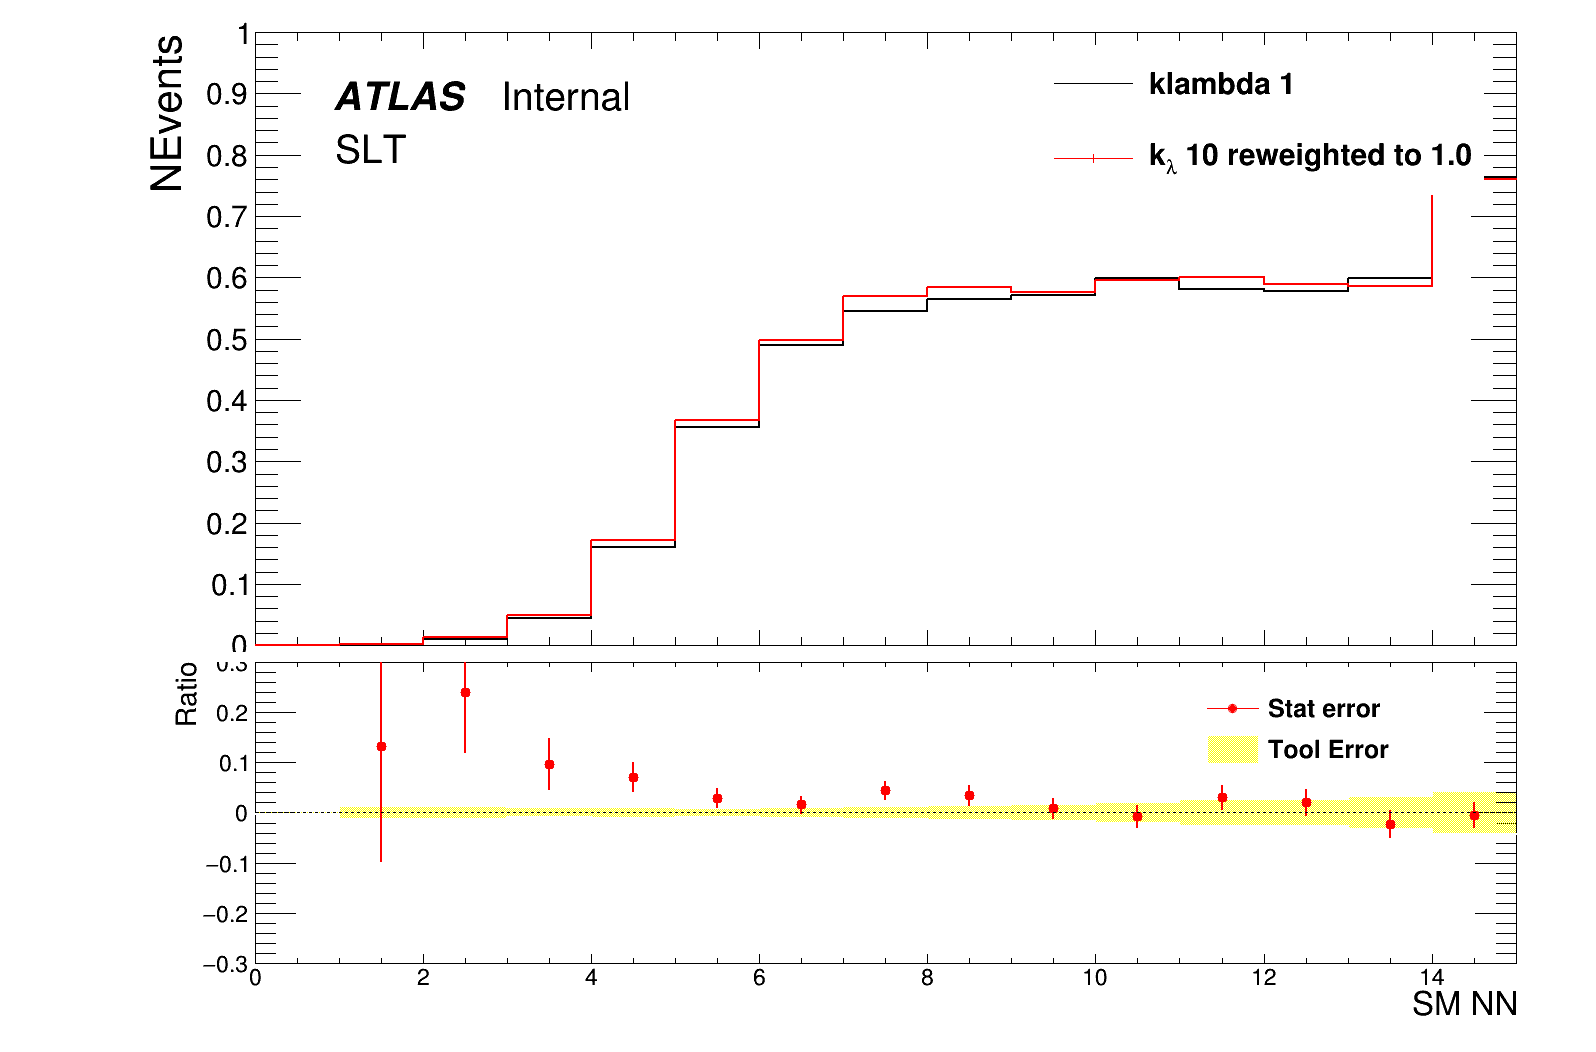
\includegraphics[width=.47\textwidth]{DiHiggs/plots/kl_SLTLimit_binning_SM_NN.png}
      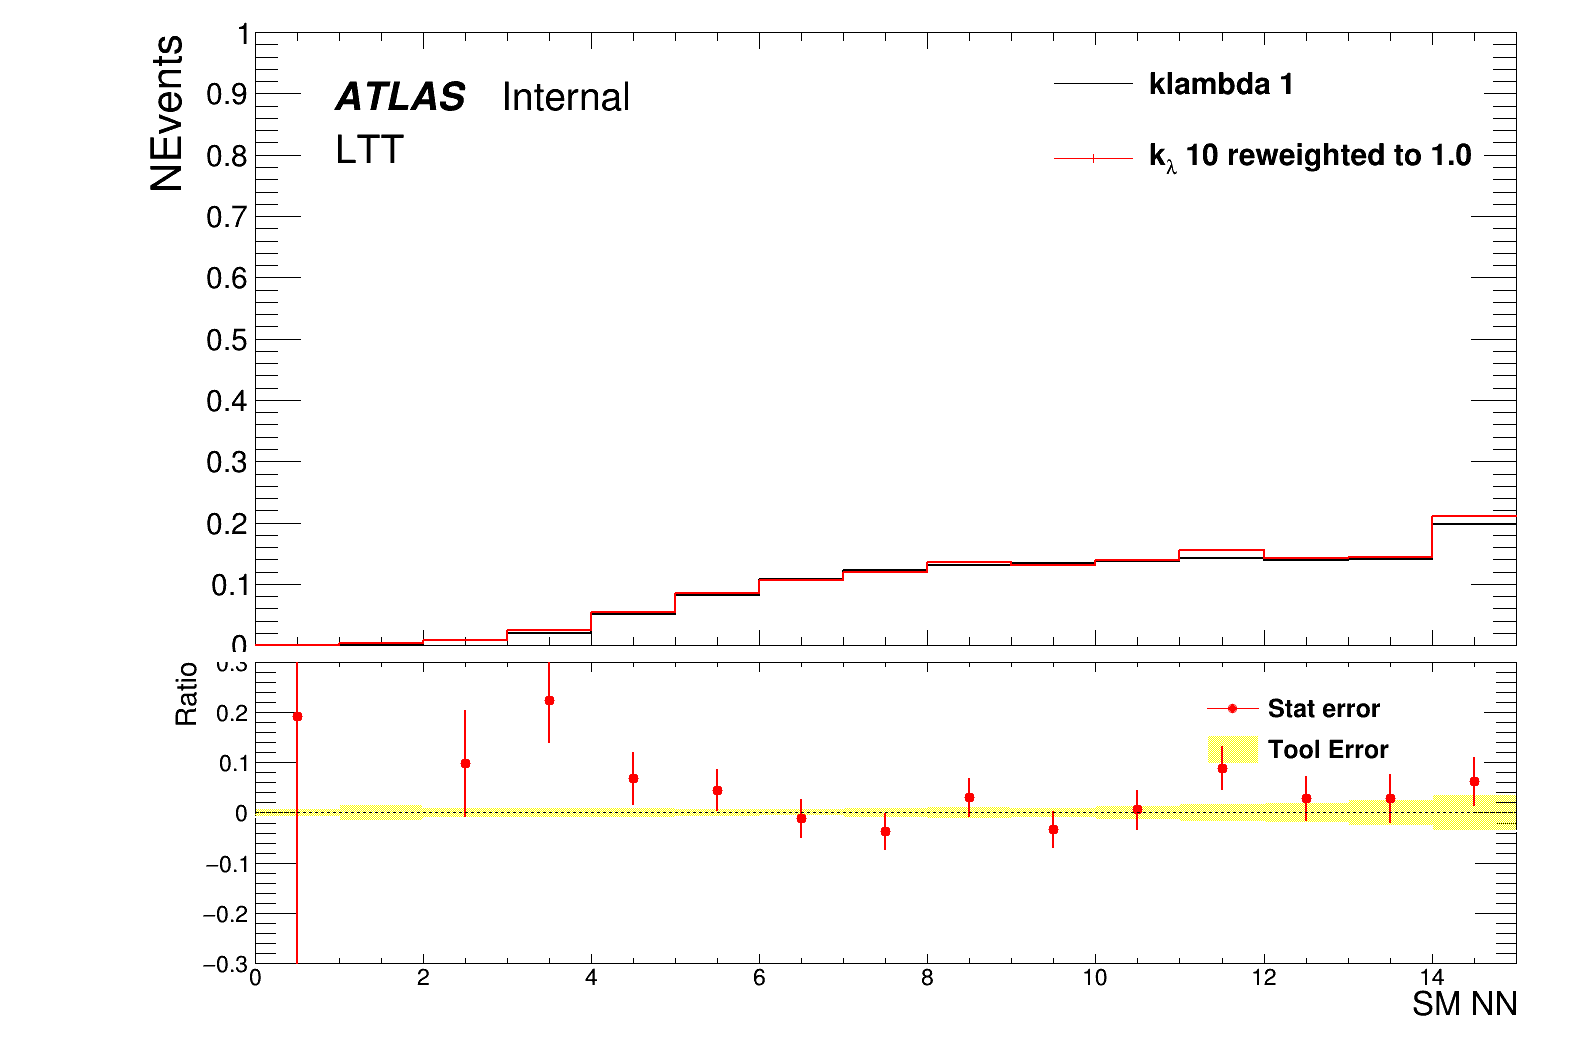
\includegraphics[width=.47\textwidth]{DiHiggs/plots/kl_LTTLimit_binning_SM_NN.png} \\
  \end{center}
  \caption{Comparison of the $\kappa_\lambda = 1$ and 10 ggF samples in the NN output for the SLT (left) and the LTT (right) channel
  The ``Tool Error'' band shows the statistical uncertainty on the applied weights, 
  originating from the limited size of the samples used to derive them.}
  \label{fig:kl_closure_bbtautau_ggf}
\end{figure}


Nevertheless, it was found that the choice of sample used as 
input for the reweighting procedure affects the obtained signal 
acceptance at different values of $\kappa_\lambda$. 
This dependence is shown in Fig.~\ref{fig:bbtautau_accxeff},
using either the generated \kl=1 or \kl=10 sample as input.
The maximal discrepancy of 3\% (SLT) or 8\% (LTT) between the measured values is applied as an uncertainty 
on the normalisation of the ggF sample after the reweighting. 
At last, the acceptance uncertainties originating from the choice 
in PS, PDF and $\alpha_s$ value or QCD scales have been derived 
for both the $\kappa_\lambda = 1$ 
and the $\kappa_\lambda = 10$ sample.
They are summarised in Tab.~\ref{tab:systematics_HHNonResSignal_AcceptanceNumbers}.
Since these could not be evaluated for all $\kappa_\lambda$ values investigated in the scan,
the greater uncertainty is applied for all signals with \kl\ not equal to 1 for each of the 
three considered sources of uncertainty.




\begin{figure}[htbp]
    \begin{center}
        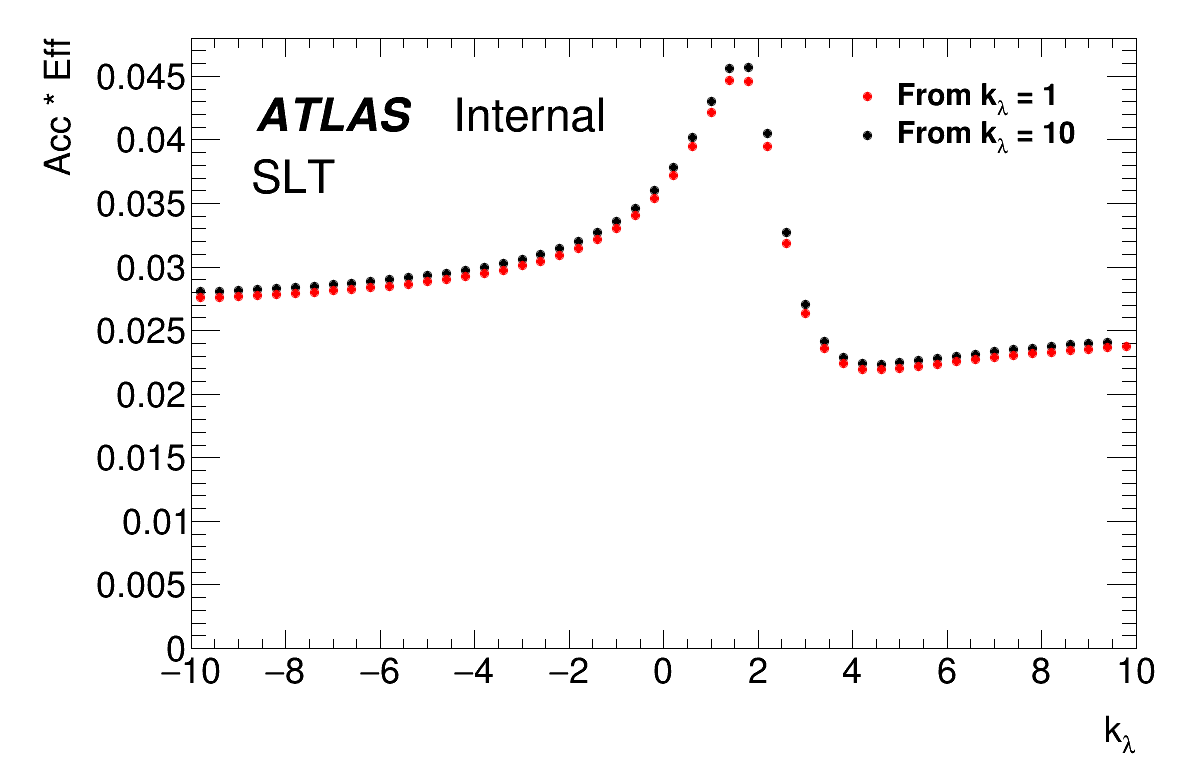
\includegraphics[width=.45\textwidth]{DiHiggs/plots/kl_SLT acc.png}
        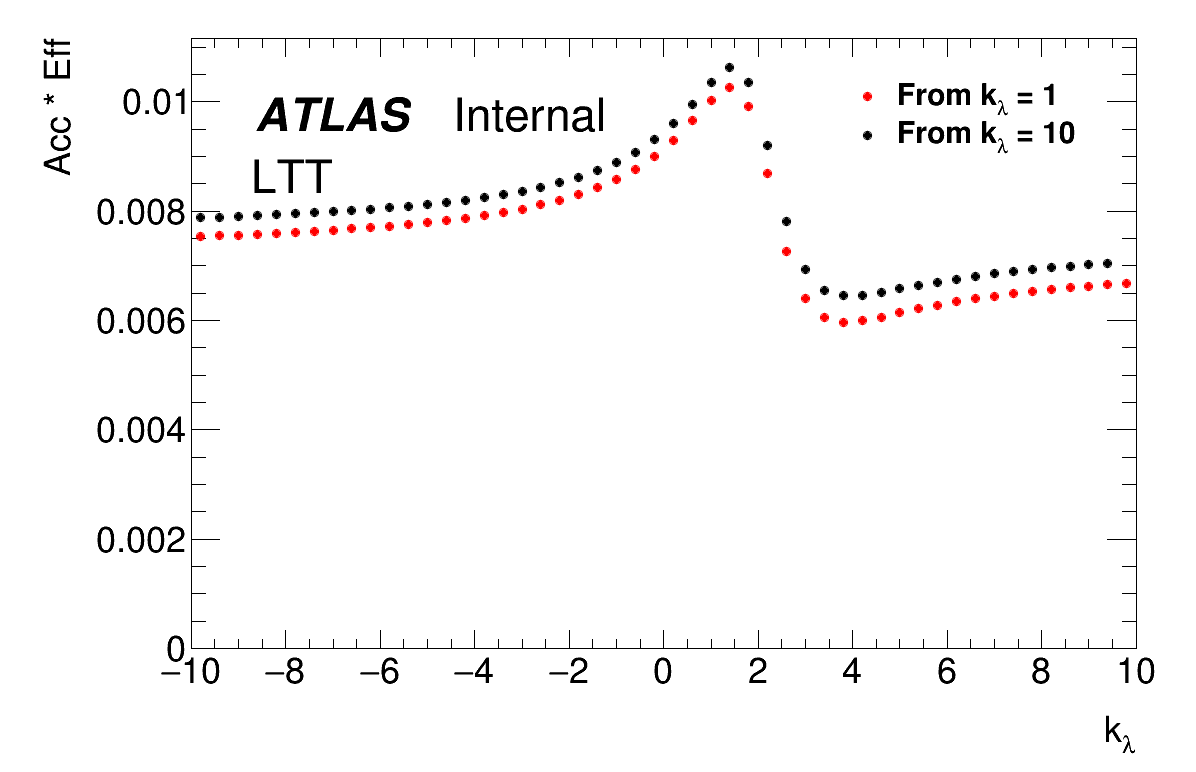
\includegraphics[width=.45\textwidth]{DiHiggs/plots/kl_LTT acc.png} \\
        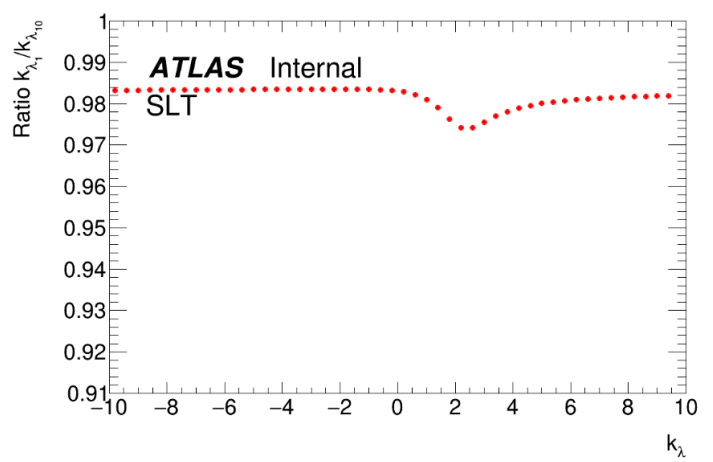
\includegraphics[width=.45\textwidth]{DiHiggs/plots/kl_scan/bbtautauSubchannels/bbtautau_kl_accxeff_slt.png}
        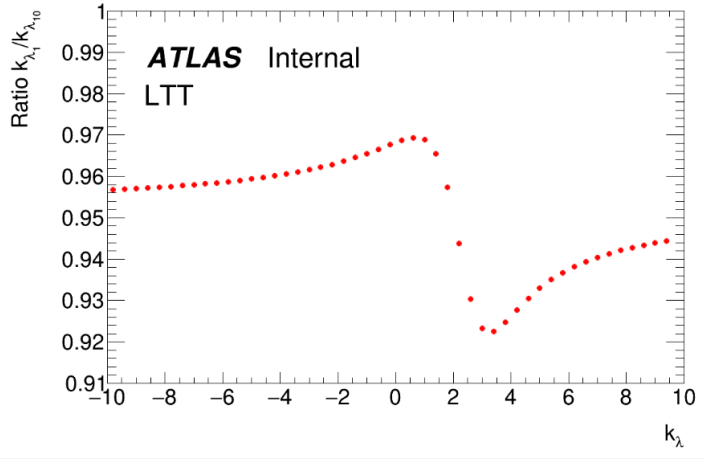
\includegraphics[width=.45\textwidth]{DiHiggs/plots/kl_scan/bbtautauSubchannels/bbtautau_kl_accxeff_ltt.png}
    \end{center}
    \caption{Comparison of acceptance $\times$ efficiency at different $\kappa_\lambda$ values depending on whether the 
    reweighting procedure is applied on the ggF sample with $\kappa_\lambda = 1$ (nominal) 
    or $\kappa_\lambda = 10$ (alternative).}
    \label{fig:bbtautau_accxeff}
\end{figure}

\begin{table}
    \centering
    \small
    \begin{tabular}{|c|c|c|c|}
        \hline
        Process & SLT & LTT & Description\\
        \hline
        SM   &  0.076 & 0.075 & PS\\
        SM  &  0.0061 &  0.0072 & PDF+$\alpha_s$\\
        SM  &  0.012 &  0.010 & Scales \\
        $\kappa_\lambda=10$  &  0.10 &  0.085 & PS\\
        $\kappa_\lambda=10$  &  0.0074 &  0.0072 & PDF+$\alpha_s$\\
        $\kappa_\lambda=10$  &  0.0087 &  0.0074 & Scales \\
        \hline
    \end{tabular}
    \caption{List and relative size of ggF HH non-resonant signal 
    acceptance uncertainties in SLT and LTT.}
    \label{tab:systematics_HHNonResSignal_AcceptanceNumbers}
\end{table}

\paragraph{Uncertainties on VBF}

As in the case of ggF, the acceptance uncertainties for VBF $HH$ production are updated.
The QCD scale and PDF+$\alpha_s$ uncertainties for the SM and $\kappa_\lambda \in \{0, 2, 10\}$
samples are listed in Tab.~\ref{tab:systematics_HHNonResSignalVBF_AcceptanceNumbers}.
Additionally, the PS uncertainty is evaluated for the SM sample and at $\kappa_\lambda = 10$.
For each of these sources of uncertainty, the largest one is used to define the respective
variation for the prediction in all non-SM cases.

An uncertainty on the closure of the linear combination of VBF samples is evaluated in both 
SLT and LTT and applied on the normalisation of the VBF sample after the linear combination. 
Four different bases of $\kappa_\lambda$ values are tested.
Closure plots are shown in Figure~\ref{fig:bbtautau_lephad_VBFclosure} in 
Appendix~\ref{sec:appendix:systs}. 
The maximal difference is found to be of 
2.2\% (SLT) and 5.8\% (LTT) 
between the multivariate discriminator distributions for the MC 
and reweighted $\kappa_\lambda$ samples, 
and it comes from the linear combination 
of VBF samples $(\kappa_\lambda = 1, 10, 0)$ to  $\kappa_\lambda=2$ in all cases.


\begin{table}[!htb]
\centering
\small
\begin{tabular}{|c|c|c|c|}
\hline
Process  & SLT & LTT & Description\\
\hline
SM  & 6.3\,\% & 2.1\,\% & PS\\
SM &  0.15\,\% &  0.23\,\% & PDF+$\alpha_s$ from NNPDF30NLO\\
SM  &  0.86\,\% &  0.63\,\% & Scales \\
$\kappa_\lambda = 0$ & 0.28\,\% & 0.21\,\% &PDF+$\alpha_s$ from NNPDF30NLO\\
$\kappa_\lambda = 0$ & 1.16\,\% & 0.91\,\% &Scales\\
$\kappa_\lambda = 2$ & 0.27\,\% & 0.23\,\% &PDF+$\alpha_s$ from NNPDF30NLO\\
$\kappa_\lambda = 2$ & 1.08\,\% & 0.89\,\% &Scales\\
$\kappa_\lambda = 10$ & 7.79\,\% & 5.73\,\% &PS\\
$\kappa_\lambda = 10$ & 0.26\,\% & 0.37\,\% &PDF+$\alpha_s$ from NNPDF30NLO\\
$\kappa_\lambda = 10$& 1.25\,\% & 0.99\,\% &Scales\\
\hline
\end{tabular}
\caption{List and relative size of VBF HH non-resonant signal acceptance uncertainties in SLT and LTT.
Table reproduced from analysis internal notes.}
\label{tab:systematics_HHNonResSignalVBF_AcceptanceNumbers}
\end{table}











\subsection{Uncertainties on fake background}
\label{sec:DiHiggs:fakesyst}
The following uncertainties are considered
for the fake background:
\begin{itemize}
  \item The statistical uncertainty on the $FF_{t\bar{t}}$, 
  $FF_\text{QCD}$ and $r_\text{QCD}$ are considered. They are
  propagated to the final estimations of the fake background.
  \item A conservative 30\% uncertainty is assigned to all non-\ttbar\
  background being subtracted from the data. This uncertainty is derived
  by varying the FF up and down by 30\% when applying on the non-\ttbar\ background
  passing the anti-ID selection. 
  A value of 50\% was also considered, but was found to be over-conservative.
  As the anti-ID selection events are dominated by fake and \ttbar\ background,
  the 30\% value is well enough to cover possible variations due to non-\ttbar\ backgrounds.  
  \item The uncertainty due to \ttbar\ modelling was estimated by the 
  difference between the fake background derived with and without the 
  \ttbar\ reweighting (more details in section~\ref{sec:DiHiggs:lephadfake}).
  An alternative approach was studied by the author, using the \ttbar\ variation samples
  used for evaluating the PS, matrix element, ISR and FSR uncertainties to replace the nominal \ttbar\ 
  samples, for deriving the FF and to be subtracted from data. The fake background derived
  using the variation samples are correlated to the corresponding ones in \ttbar\ modelling 
  uncertainties estimations. 
  The PNN score distributions of the fake background derived using the variation samples 
  are shown in Appedix~\ref{sec:appendix:systs}, Figures~\ref{fig:ttbarsyst_lephad_Fakes_SLT_PNN}-~\ref{fig:ttbarsyst_lephad_Fakes_LTT_PNN_ratio_fullsim}.
  
  These two methods were compared by the author, where the first one was adopted at last
  due to the variation is observed to be higher and hence covering all fake background derived
  using variation samples. In addition, these two methods are accounting for the same source
  of uncertainty originating from the MC modelling of the \ttbar\ background, therefore
  only the first method was used to avoid double counting. 
  \item  The $r_\text{QCD}$ is highly sensitive to the \ttbar\ background. 
  Given the fact that the $FF_\text{QCD}$ and $FF_{t\bar{t}}$ is very similar, 
  the $r_\text{QCD}$ in practice does not have big impact on the combined fake factor. 
  Therefore the uncertainty on $r_\text{QCD}$ is estimated by varying the value from 0 to 0.5. 
  The impact of assigning such a conservative uncertainty was checked and was found to be
  very small. 
   
\end{itemize}
